%%%%%%%%%%%%%%%%%%%%%%%%%%%%%%%%%%%%%%%%%%%%%%%%%%%%%%%%%%%%%%%%%%%%%%%%
%                                                                      %
% LaTeX, FIIW thesis template                                          %
%                                                                      %
%%%%%%%%%%%%%%%%%%%%%%%%%%%%%%%%%%%%%%%%%%%%%%%%%%%%%%%%%%%%%%%%%%%%%%%%
\documentclass[11pt,a4paper]{report}
% Indien je je thesis recto-verso wil afdrukken gebruik je onderstaande opties i.p.v. bovenstaande
%\documentclass[11pt,a4paper,twoside,openright]{report}

\usepackage[a4paper,left=3.5cm, right=2.5cm, top=3.5cm, bottom=3.5cm]{geometry}
\usepackage[dutch]{babel}
\usepackage{graphicx}
%\usepackage[latin1]{inputenc}           % om niet ascii karakters rechtstreeks te kunnen inputten
\usepackage[utf8]{inputenc}            % commentarieer deze regel uit als je utf8 encoded files gebruikt in plaats van latin1
\usepackage{natbib}
\usepackage{listings}             		% voor het weergeven van broncode
\usepackage{booktabs}
\usepackage{verbatim}					% weergeven van code, commando's, ...
\usepackage[hidelinks]{hyperref}					% maak PDF van de thesis navigeerbaar
\usepackage{url}						% URL's invoegen in tekst met behulp van \url{http://}
\usepackage[small,bf,hang]{caption}     % om de captions wat te verbeteren
\usepackage[final]{pdfpages}            % gebruikt voor het invoegen van het artikel in pdf-formaat
\usepackage{pslatex}					% andere lettertype's dan de standaard types
\usepackage{lipsum}
\usepackage{textgreek}
\usepackage{csquotes}
\usepackage{color}
\usepackage{listings}
\lstset{numbers=right,  
                breaklines=true,
                numbersep=5pt,
                caption=\lstname,
                captionpos=b,
                xleftmargin=15pt} 
\lstset{language=Python} 
\usepackage{amsmath}					%wiskundige formules
\usepackage{sectsty}					% aanpassen van de fonts van sections en chapters
\usepackage[]{tocbibind}	% Bibliography mee in de ToC
\setcounter{tocdepth}{1}

\allsectionsfont{\sffamily}
\chapterfont{\raggedleft\sffamily}

\usepackage{float}                      % De optie H voor de plaatsing van figuren op de plaats waar je ze invoegt. bvb. \begin{figure}[H]
%\usepackage{longtable}					% tabellen die over meerdere pagina's gespreid worden
%\usepackage[times]{quotchap}           % indien je fancy hoofdstuktitels wil
%\usepackage[none]{hyphenat}
%\usepackage{latexsym}
%\usepackage{amsmath}
%\usepackage{amssymb}

% MFA: zet zoekpad voor figure
\graphicspath{{fig/}}

\usepackage{fiiw}
% \usepackage{fiiw_eng} % For the english version (also change last page at the bottom of this file!

%door onderstaande regels in commentaar te zetten, of op false, kan je pagina's weglaten
%bijvoorbeeld het weglaten van een voorwoord, lijst met symbolen, ...
%%%%%%%%%%%%%%%%%%%%%%%%%%%%%%%%%%%%%%%%%%%%%%%%%%%%%%%%%%%%%%%%%%%%%%%%%%%%%%%%%%%%%%%%
%voorwoord toevoegen?
%\acknowledgementspagetrue
%\acknowledgements{voorwoord}			%.tex file met daarin het voorwoord

%samenvatting toevoegen
%\summarypagetrue
%\summary{samenvatting}					%.tex met daarin de samenvatting

%abstract toevoegen?
%\abstractpagetrue
%\abstracts{abstract}					%.tex file met daarin het abstract
%lijst van figuren toevoegen?
\listoffigurespagetrue
%lijst van tabellen toevoegen?
\listoftablespagetrue
%lijst van symbolen toevoegen?
%\listofsymbolspagetrue
%\listofsymbols{symbolen}				%.tex file met daarin de lijst van symbolen
%lijst van afkortingen toevoegen?
\listofabbrevspagetrue
\listofabbrevs{afkortingen}				%.tex file met daarin de lijst van symbolen

%informatie over het eindwerk, de promotor, ...
%%%%%%%%%%%%%%%%%%%%%%%%%%%%%%%%%%%%%%%%%%%%%%%
\opleiding{E-ICT}
\afdeling{ICT}

\campus{denayer} 



\title{Wandelen door kristallen}
\subtitle{Blender als kristallografische visualisatietool}
\forenameA{Jarrit}
\surnameA{Boons}
\forenameB{}
\surnameB{}

\academicyear{2018 - 2019}

\promotorA[Promotor]{Ann Phillips}
\promotorB[Co-promotor]{prof. Christine E. A. Kirschhock}

\begin{document}
\selectlanguage{dutch}
\preface

%%%%%%%%%%%%%%%%%%%%%%%%%%%%%%%%%%%%%%%%%%%%%%%%%%%%%%%%%%%%%%%%%%% 
%                                                                 %
%                           INLEIDING                             %
%                                                                 %
%%%%%%%%%%%%%%%%%%%%%%%%%%%%%%%%%%%%%%%%%%%%%%%%%%%%%%%%%%%%%%%%%%% 


\chapter{Inleiding}
Dit hoofdstuk omschrijft de context waarin deze thesis zich zal afspelen en vormt het fundament van deze scriptie. Om de rest van deze thesis te begrijpen is het van belang dit hoofdstuk grondig te lezen. 
\\
De eerste sectie van dit hoofdstuk schetst onder welke onderzoeksdomeinen deze thesis kan worden ondergebracht. De tweede sectie beschrijft het probleem waarop deze thesis een oplossing zal trachten te bieden. Het algemene doel van deze thesis is het vinden en uitwerken van deze oplossing, dit doel zal verder worden opgedeeld in verschillende, kleinere, doelstellingen. In sectie vier worden deze doelstellingen geformuleerd als onderzoeksvragen  bestaande uit een hoofdvraag en enkele deelvragen. Ten slotte is er nog een vijfde sectie waarin de opbouw van deze scriptie wordt beschreven. In een laatste sectie wordt dit hoofdstuk samengevat in een beknopte conclusie.

\section{Situering van het onderzoek}
Kristallografie is een tak van de wetenschap met als hoofdrol een eerder klein object, een kristal. Kristallen kunnen gezien worden als een puzzel van atomen. De stukjes van zo een puzzel kunnen verschillende chemische elementen zijn, maar evengoed allemaal dezelfde. Wat de kristallen zo uniek maakt is hoe deze zijn opgebouwd. De opbouw bepaalt allerhande eigenschappen van dat bepaalde kristal. De complexiteit van kristallen kan oplopen tot op het punt waarop het bijna onmogelijk wordt deze in woorden te beschrijven en zelfs nog moeilijker deze te interpreteren. Dit is waar computertechnologie aan te pas komt. 
\\
Sinds enkele decennia zijn wetenschappers in staat kristalstructuren om te zetten in een digitaal formaat dat leesbaar is door zowel mensen als computers, het CIF-formaat (zie later). Dankzij dit standaardformaat is het mogelijk geworden de structuur van kristallen te lezen en te delen zonder kans op misinterpretatie, en biedt het computers de mogelijkheid zelfs de meest complexe kristalstructuren naar een driedimensionaal beeld om te zetten. Het 3D visualiseren van kristallen geeft wetenschappers meer inzicht en geeft meer mogelijkheden om hun kennis over te brengen. Dit alles heeft geleid tot een nauwe samenwerking tussen kristallografie en computerwetenschappen om de wereld van de kristallografie tot leven te brengen.


\section{Probleemstelling}
De programma’s die op dit moment door wetenschappers worden gebruikt bij het 3D visualiseren van kristallen bieden nog lang niet de vrijheid en aanbod aan features welke sommige hedendaagse 3D-software en game-engines te bieden hebben. Het van de grond opbouwen van 3D visualisatiesoftware of zelfs reeds bestaande software aanpassen is een enorme taak en slechts weinig wetenschappers hebben hier de tijd noch de technische knowhow voor. Daarnaast is het moeilijk om programmeurs te vinden die de nodige kennis bezitten over kristallografie en kristalstructuren of zich hierin willen verdiepen.  
\\
Het gebruiken van Blender als software om kristallen te visualiseren is een stap in de goede richting. Deze open source software laat, mits enige kennis van het programma, toe driedimensionale figuren te creëren en te bekijken. Het groot aantal features in Blender biedt de gebruiker veel vrijheid aan, wat ontbreekt in hedendaagse kristalvisualisatiesoftware. 3D objecten aanmaken en bekijken doet men via de grafische interface van Blender of met behulp van een script. Het gebruiken van scripts is erg interessant voor de gebruiker omdat deze hiermee langdradige of repetitieve taken kan laten uitvoeren. 
\\
In de context van kristallografie laat dit toe dat een kristal, bestaande uit een groot aantal atomen, niet meer manueel moet getekend worden. Helaas biedt dit geen volledige oplossing voor het probleem, voor elk kristal moet er nog steeds een apart script worden geschreven waarin alle informatie van dat kristal staat. Het scripten in Blender wordt gedaan aan de hand van Python en de API van Blender (zie verder). Hierdoor is het schrijven van scripts niet vanzelfsprekend en zonder enige voorkennis onbegonnen werk.

\section{Doelstelling}
Het algemene doel van dit werk is het ontwerpen van een interface die kristalstructuren kan visualiseren in het voornoemde open source programma, Blender. Eens dit bereikt is, zijn de mogelijkheden virtueel eindeloos. 
\\
Een van de problemen bij het visualiseren van een kristal met scripten in Blender is dat voor elke kristalstructuur een nieuw script moet worden geschreven. De interface moet gezien worden als een black box met als input de beschrijving van een kristalstructuur en de driedimensionale voorstelling hiervan als output. Dit stelt de nood aan een input die interpretabel moet zijn door een computer en die in eerste instantie in eenzelfde formaat is om de omvang van het programma te beperken. Dit kan nadien nog uitbereid worden zodat verschillende formaten kunnen worden ingelezen. De eerste doelstelling is dus een keuze te maken van formaat dat er kan ingelezen worden door de interface.  
\\
De volgende stap in het ontwerpproces van de interface is het schrijven van een functie die in staat is het eerder gekozen formaat in te lezen en om te zetten naar bruikbare data. Afhankelijk van de complexiteit en striktheid van het formaat kan het ontwerpen van dit soort routines erg tijdrovend zijn. Het is mogelijk dit te vermijden door op zoek te gaan naar een reeds bestaande Python modules met een gelijkaardige werking en deze, indien mogelijk, te implementeren in de interface. Eens het formaat kan worden ingelezen, moet nodige informatie worden opgeslagen. Python biedt de mogelijk aan om gebruik te maken van classes, wat toelaat de kristaldata op te slaan in zelfgecreëerde datastructuren, wat de uiteindelijke dataverwerking zal vereenvoudigen. 
\\
De Blender API geeft de gebruiker een keuze uit een immens aantal functies. Dit zorgt er echter voor dat scripten in Blender zonder de nodige voorkennis erg complex kan worden. Een belangrijk onderdeel van deze scriptie is dan ook het verdiepen in de API van Blender en alle mogelijkheden die deze biedt. Met de nodige kennis van de functies wordt het mogelijk de gemaakte datastructuren driedimensionaal te visualiseren in Blender. Enkele basisfeatures die de interface moet hebben is een manier om elementen te onderscheiden met behulp van kleur, automatisch bindingen maken tussen atomen op basis van hun onderlinge afstand en meerdere eenheidskristallen naast elkaar kunnen tekenen.
\\
Ten slotte zullen de limieten van Blender getest worden in de context van het wetenschappelijk onderzoek rond kristallen.  


\section{Onderzoeksvragen}
De doelstellingen uit vorige sectie kunnen worden geformuleerd als onderstaande onderzoeksvragen.
\\
Hoofdvraag:
\\
Is het mogelijk een interface te ontwerpen die in staat is kristalstructuren driedimensionaal te visualiseren in Blender?
\\
Deelvragen:
\\
Wat is de meest efficiënte methode om een kristalstructuur om te zetten in verwerkbare data?
\\
Wat is de beste manier om kristaldata te visualiseren in Blender?
\\
(extra) Hoe ver kan Blender gepushed worden als 3D visualisatiesoftware voor kristallen? 


\section{Structuur van de tekst}
Het eerste hoofdstuk geeft een inleiding tot het algemene onderwerp van deze thesis. Hier zal onder andere de probleemstelling en het doel van dit onderzoek worden besproken. Dit hoofdstuk heeft als doel een kort overzicht te geven over de verdere inhoud van deze scriptie.  
\\
In het tweede hoofdstuk wordt de literatuurstudie besproken. Dit onderdeel van de tekst verdiept zich in kristallografie, het gebruikte formaat van kirstalbeschrijving, reeds bestaande visualisatie software, de parser en tot slot Blender en de Blender API. Het doel van dit hoofdstuk is inzicht geven in het theoretische aspect van de thesis en de nodige kennis verschaffen over de gebruikte technologieën.
\\
In het derde hoofdstuk wordt het ontwerpproces beschreven. Hier kunnen de stappen worden gevolgd die zijn ondernomen in het opbouwen van de interface. Er wordt op een oppervlakkige manier gekeken naar de opbouw van het programma om het globale overzicht te behouden. Dit hoofdstuk schetst de algemene structuur van het programma en de gedachtegang tijdens het ontwerpen hiervan.
De inhoud van het vierde hoofdstuk beschrijft de structuur van de ontworpen interface en hoe deze juist werkt. Deze tekst geeft een technische kijk op het programma en overloopt bepaalde onderdelen van de geschreven code in meer detail. Er wordt onder andere dieper ingegaan op de werking van de Blender API en de CIF-parser.
\\
Hoofdstuk vijf kijkt in detail naar de output van het programma. Er wordt dieper ingegaan op de resultaten, complicaties, mijlpalen en gemaakte fouten. 
De eindconclusie van de thesis wordt besproken in hoofdstuk zes. Alle relevante informatie uit voorgaande hoofdstukken wordt hier opgesomd om een duidelijk overzicht te geven over het volledige onderzoek. De resultaten worden in dit hoofdstuk nogmaals kort overlopen om zo tot een uiteindelijk besluit te komen betreffende dit eindwerk.
\\


\section{Conclusie}
Dit hoofdstuk gaf een overzicht over het onderwerp en de omvang van deze thesis, kaartte de probleemstelling aan en formuleerde enkele onderzoeksvragen die als rode draad doorheen deze tekst dienen. Met de kennis uit dit hoofdstuk zal de stap naar zowel de literatuurstudie als naar het meer praktische onderdeel van dit onderzoek minder groot zijn.

%%%%%%%%%%%%%%%%%%%%%%%%%%%%%%%%%%%%%%%%%%%%%%%%%%%%%%%%%%%%%%%%%%% 
%                                                                 %
%                            CHAPTER                              %
%                                                                 %
%%%%%%%%%%%%%%%%%%%%%%%%%%%%%%%%%%%%%%%%%%%%%%%%%%%%%%%%%%%%%%%%%%% 

\chapter{Literatuurstudie}

Vooraleer een oplossing  kan worden ontworpen voor een probleem is het van belang de nodige informatie te verzamelen over de huidige staat van het probleem en eventuele reeds bestaande oplossingen. In dit hoofdstuk zal er onder andere worden gekeken naar de technologieën die op dit moment in de wetenschap gebruikt worden en welke technologieën mogelijk een oplossing kunnen bieden voor het probleem. 
\par
Het lezen van dit hoofdstuk is aangeraden aangezien het enkele belangrijke begrippen en technologieën beschrijft waarnaar zal worden verwezen in dit onderzoek. Het is echter mogelijk dit hoofdstuk over te slaan als deze informatie reeds gekend is of als de theorie achter het proces minder van belang is.
\par
Omdat dit onderzoek zich deels afspeelt binnen de wereld van kristallografie, een specifieke tak van de wetenschap, zal de eerste sectie van dit hoofdstuk gewijd worden aan het overlopen van enkele begrippen die van belang zullen zijn in het verdere verloop van het onderzoek. Daar kristallografie een eerder complexe wetenschap is, zal deze tekst een vereenvoudigde beschrijving zijn. Voor een meer accurate beschrijving wordt er verwezen naar de literatuur waarop deze sectie gebaseerd is \citep*{CRYS1}. De tweede sectie zal het Crystallographic Information File of CIF-formaat beschrijven. Dit tekstformaat ligt aan de basis van het digitaliseren van kirstalstructuren en zal gebruikt worden bij het inlezen van kristaldata. In de derde sectie wordt gekeken naar welke programma’s op dit moment worden gebruikt bij het visualiseren van kristallen en hoe deze werken. De vierde sectie kijkt naar enkele reeds bestaande CIF-parsers en of deze al dan niet kunnen gebruikt worden in dit onderzoek. Sectie vijf zal zich verdiepen in de werking van Blender en de Blender API. In de zesde en laatste sectie wordt een conclusie getrokken uit de verkregen informatie.


\section{Kristallografie}

\subsection{Wat is kristallografie}
Kristallografie kan beschreven worden als de studie van materie in een kristallijne staat en houdt zich onder andere bezig met de synthese en opbouw van kristallen en hun fysische en chemische eigenschappen. Eerder in dit hoofdstuk werd kristallografie beschreven als een specifieke tak van de wetenschap, het is echter vermeldenswaardig dat dit een erg omvattende studie is. Kristallen komen namelijk voor in vrijwel elk ander wetenschappelijk domein. Tabel[2.1] toont enkele voorbeelden van kristallen en de respectievelijke tak van de wetenschap waar deze onder vallen.
\par
In dit onderdeel zullen verder enkel de kristallografische begrippen worden beschreven die binnen de omvang van deze thesis vallen.  
\par
\begin{table}
\caption{Kristallen in wetenschappelijke takken}
\begin{tabular}{@{}ccccl@{}}
\toprule
\multicolumn{1}{c}{\textbf{Biologie}} & \multicolumn{1}{c}{\textbf{Chemie}} & \multicolumn{1}{c}{\textbf{Farmacologie}} & \multicolumn{1}{c}{\textbf{Geologie}} &  \\ \midrule
proteïnes                              & rubber                               & alle vaste medicijnen                      & alle mineralen                         &  \\
polysacharides                         & benzeen                              & vitamines                                  & metalen                                &  \\
beenderen                              & naftaleen                            &                                            &                                        &  \\ \bottomrule
\end{tabular}
\end{table}

\subsection{De eenheidscel}
Alle kristallen zijn gedefinieerd als een periodische schikking van atomen, ionen of moleculen. Het opbouwen van een kristal wordt gedaan aan de hand van roosterpunten. Een aantal roosterpunten op een lijn met een gelijke onderlinge afstand wordt een roosterlijn genoemd, een verzameling van evenwijdige roosterlijnen met eenzelfde onderlinge afstand is een roostervlak. Ten slotte kan dit worden herhaald in een derde dimensie en wordt er een roosterruimte gevormd, welke in zwart getekend staat op Figuur[2.1]. Een roosterruimte kan in essentie zo groot zijn als het beschreven kristal. Zoals eerder ook gezegd is een kristal periodisch, dit wil zeggen dat er enkel moet gekeken worden naar het kleinste unieke volume van een kristal. Dit uniek volume valt volledig binnen de roosterruimte beschreven door de eerste acht roosterpunten. Het volledige kristal kan worden opgebouwd door de translatie van deze eenheidscel in 3 richtingen in de ruimte. Een kristal bestaat gewoonlijk uit een groot aantal van deze eenheidscellen.
\par
Geometrisch gezien bevat een eenheidscel 3 paar evenwijdige parallellogrammen als omhullende vlakken en kan het beschreven worden aan de hand van 6 variabelen, welke de roosterparameters worden genoemd.  De parameters a, b en c bepalen de lengte tussen de roosterpunten volgens de drie assen van de roosterruimte . De drie resterende  variabelen worden gebruikt om de hoeken tussen deze assen te beschrijven en worden \textalpha, \textbeta{} en \textgamma{} genoemd. Deze variabelen staan ook aangeduid op Figuur[2.1] met de eenheidscel in rood. 

\begin{figure}
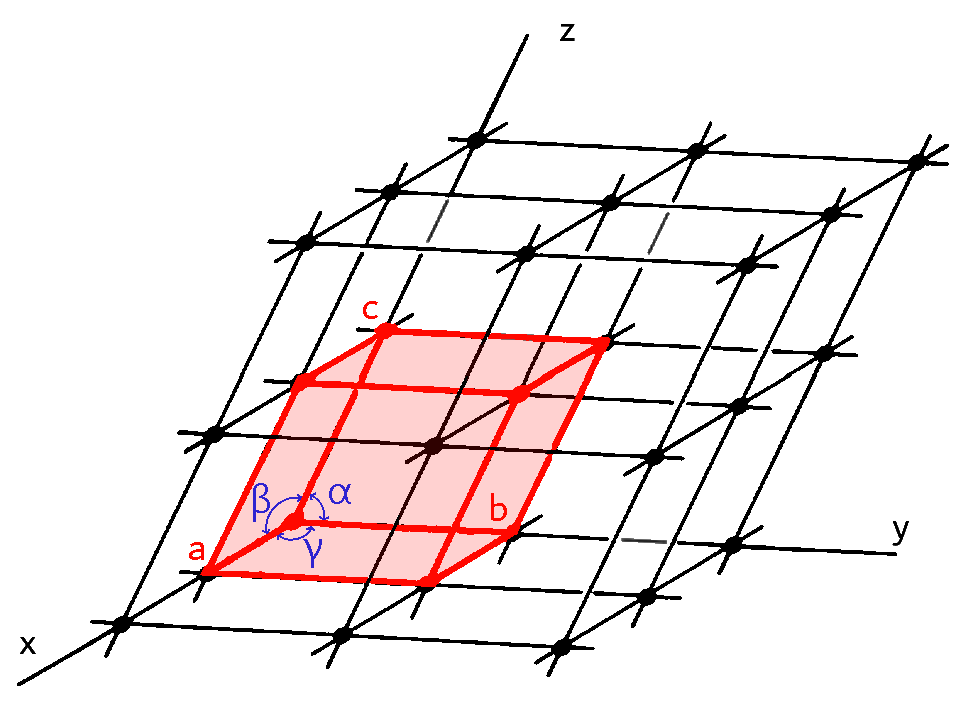
\includegraphics[scale=0.3]{roosterruimte.png}
\caption{Voorstelling van een eenheidscel in de roosterruimte \citep*{CRYS1}}
\end{figure}

\subsection{Classificatie van kristalroosters}
De vorm van de eenheidscel van een kristal is niet willekeurig, omdat dit volume de ruimte volledig moet kunnen vullen. Mogelijke types van eenheidscellen kunnen worden herleid op basis van de vorm van het vlak dat deze beschrijft, zie kolom a van Figuur[2.2]. De driedimensionale eenheidscel kan dan worden verkregen door de extrusie van dit vlak in de derde dimensie, zie kolom c van Figuur[2.2]. Zo bestaan er exact zes coördinaatsystemen, gebaseerd op de restricties van de roosterparameters. Deze vormen de basis voor de classificatie in kristalfamilies en krijgen de naam: kubisch, tetragonaal, orthorhombisch, monoclinisch, triclinisch, en hexagonaal. Deze worden weergegeven in kolom b van Figuur[2.2]. 

\par 
Vertrekkende van de mogelijke coördinaatsystemen en rekening houdend met mogelijke symmetrieën ontstaan er zeven kristalsystemen, zie kolom a van Figuur[2.3]. Hierbij wordt het hexagonale coördinatenstelsel verder opgesplitst in het trigonale en hexagonale kristalsysteem, afhankelijk van de aanwezigheid van een drie- of zesvoudige symmetrie. De zeven resulterende primitieve eenheidscellen beschrijven  voor de zeven kristalsystemen alle mogelijke eenheidstranslaties in de richtingen van x, y en z. Dit wil zeggen dat een atoom of molecule op een positie (x,y,z) ook altijd aanwezig zal zijn in de richtingen van x, y en z als de afstand identiek is aan een veelvoud van de eenheidstranslaties in deze richtingen.

\begin{figure}[H]
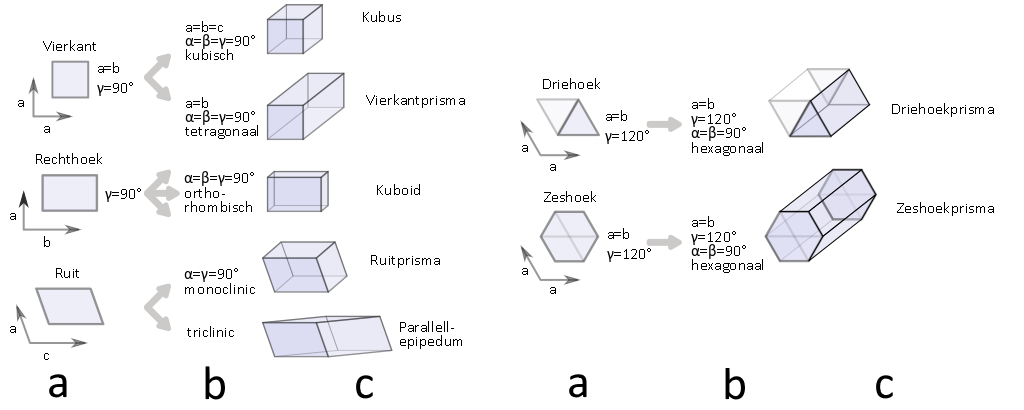
\includegraphics[scale=0.6]{families.png}
\caption{De 6 kristalfamilies}
\end{figure}

\par   
De Franse natuurkundige Bravais \citep*{BRAV} geeft een extra indeling op basis van mogelijke translaties binnen de eenheidscel, welke in overeenkomst met de symmetrievoorwaarden van de kristalsystemen zijn. Dit leidt tot de 14 Bravaisroosters, ook wel gecentreerde roosters genoemd welke worden beschreven met een letter. 
De eerste wordt de primitieve genoemd en krijgt de letter P toegekend. Bij deze bestaan alleen de eenheidstranslaties. Het rooster bevat alleen roosterpunten op de 8 hoeken van de cel.
\\
Het tweede gecentreerde rooster noemt men grondvlakgecentreerd. Deze heeft naast de eenheidstranslaties ook een centrering in een vlak. Elk deeltje kan ook teruggevonden worden over een translatie van een halve lengte langs twee assen. Er kan sprake zijn van A, B of C centrering als de verschuiving langs de diagonaal van respectievelijk het bc-, ac- of ab- vlak aanwezig is. Ondanks dit verschil worden ze niet als aparte gecentreerde roosters beschouwd.   
\\
Wanneer er extra roosterpunten liggen in elk van voorgaande vlakken spreekt men van een vlakgecentreerd of F-rooster. 
\\
Ten slotte kan er zich, naast de roosterpunten op de hoeken, ook een in het centrum van het rooster bevinden, in dit geval wordt er van een ruimtegecentreerd of I-rooster gesproken. 
\\
In het geval van het trigonale kristalsysteem bestaat er een speciale vorm van centrering in overeenkomst met de drievoudige symmetrie, welke R-centrering genoemd wordt. Kolom b van Figuur[2.3] geeft de 14 resulterende Bravaisroosters weer, dit zijn alle mogelijke vormen dat een kristal kan aannemen.
 
\begin{figure}[H]
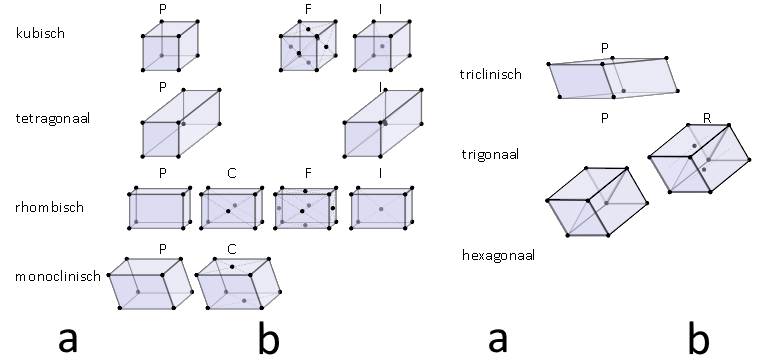
\includegraphics[scale=0.6]{Bravais.png}
\caption{De 14 Bravaisroosters en hun kristalsystemen}
\end{figure}

\subsection{Ruimte- en puntgroepen}
Dit concept is vrij complex en minder van belang voor dit onderzoek. Omdat gerelateerde termen in het verloop van deze tekst aan bod komen is het toch best deze beknopt toe te lichten. In deze literatuurstudie zal de exacte theorie hierachter niet in detail beschreven worden, maar enkel wat er van belang is voor het begrijpen van deze thesis.

\par
Puntgroepen wijzen op de innerlijke symmetrie van een roosterpunt. Een puntgroep kan gezien worden als een verzameling van symmetrieoperaties. Een symmetrieoperatie wordt als een manipulatie van een object beschouwd welke het object in zijn oorspronkelijke vorm transformeert. Naast de identiteit van een object met zichzelf zijn er vier verschillende soorten van symmetrieoperaties: spiegeling in een vlak , rotatie rond een as, inversie en de combinatie van een spiegeling en een inversie, wat een draai-inversie wordt genoemd. In totaal bestaan er 32 kristallografische puntgroepen, welke in overeenkomst zijn met de symmetrievoorwaarden van de 7 reeds besproken kristalsystemen. 

\par
Ruimtegroepen kijken niet enkel naar innerlijke symmetrie maar ook naar de symmetrie van de kristalstructuren en worden verkregen door de puntgroepen toe te passen op de 14 reeds gekende Bravaisroosters. Dit leidt tot in theorie 448 combinaties, maar door de gelijkenis tussen sommige is dit nummer terug te brengen naar een totaal van 230 ruimtegroepen. Dit heeft als gevolg dat er 230 verschillende manieren bestaan om deeltjes te ordenen in een eenheidscel. Als gevolg kan elk kristal altijd in een van deze ruimtegroepen beschreven worden. 

\subsection{Beschrijving van een kristal}
Met voorgaande informatie in het achterhoofd is het mogelijk een kristalstructuur te beschrijven. De enige informatie die hiervoor nodig is, is de ruimtegroep, het gebruikte coördinaatsysteem en de mogelijke centrering die alle symmetrieoperaties definieert. Vervolgens worden de roosterparameters van de eenheidscel gegeven en de lijst van elementen waarop deze symmetrieoperaties geldig zijn. Ten slotte kan er ook een lijst worden gegeven van alle atomen die niet door het uitoefenen van de gegeven symmetrieoperaties geplaatst kunnen worden. Deze symmetrieonafhankelijke atomen in hun elementaire cel worden een asymmetrische eenheid genoemd. Met voorgaande gegevens kan elk mogelijk kristal afgebeeld en beschreven worden. 

\subsection{Het fractionele coördinatensysteem}
De positie van atomen binnen het eenheidskristal wordt meestal beschreven aan de hand van zijn x-, y- en z-waarden. Deze waarden stellen steeds hun relatieve positie voor ten opzichte van de respectievelijk a- b- en c-waarden van de roosterparameters, vandaar de naam fractioneel, en liggen steeds tussen nul en een. Het gebruik van het fractionele systeem heeft als groot voordeel dat het erg eenvoudig te interpreteren is, zo hoeft er geen rekening gehouden te worden met de hoeken tussen de assen van het eenheidskristal. Een element met waarden ($\frac{1}{2}$,$\frac{1}{2}$,$\frac{1}{2}$) ligt dus bijvoorbeeld in het midden van het kristal, terwijl een met waarden (1,1,1) het hoekpunt van het rooster inneemt dat zich diagonaal tegenover de oorsprong van het rooster bevindt, Figuur[2.4].
\par
\begin{figure}[H]
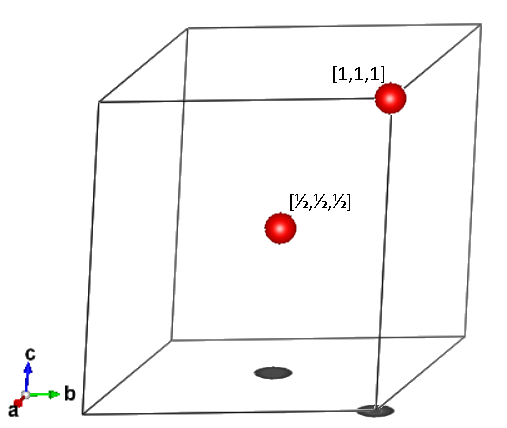
\includegraphics[scale=0.5]{FractionalExample.png}
\caption{Twee elementen in een rooster met hun fractionale coördinaten}
\end{figure}
\par
Het fractionele coördinatensysteem brengt natuurlijk ook enkele nadelen met zich mee. Om een kristal, en zijn elementen, weer te geven als een driedimensionaal figuur is er nood aan coördinaten volgens het orthogonale systeem, hiervoor kunnen de fractionele coördinaten dus niet gebruikt worden. Er zouden enkel waarden tussen nul en één kunnen verkregen worden wat telkens zou leiden tot een kubusvormig kristal. Deze foute dimensionering kan worden vermeden door deze te vermenigvuldigen met de lengte van hun respectievelijke as van het kristalrooster. Dit laatste biedt slechts deels een oplossing voor de omzetting van het fractioneel naar het orthogonaal coördinatensysteem en is enkel van toepassing voor kubische, tetragonale en orthorhombische kristalroosters aangezien deze uitsluitend bestaan uit rechte hoeken. Om een algemene formule op te stellen die gebruikt kan worden bij deze conversie moet er ook rekening gehouden worden met de hoeken tussen de assen van het kristalrooster. De algemene formule wordt voorgesteld als een matrix en ziet er voor een kristal met roosterparameters a, b, c, \textalpha, \textbeta{} en \textgamma{} uit als volgt. 
\par
\[
\begin{bmatrix}
    a & b \cdot cos(\gamma) & c \cdot cos(\beta) \\
    0 & b \cdot sin(\gamma) & c \cdot \dfrac{cos(\alpha)-cos(\beta) \cdot cos(\gamma)}{sin(\gamma)}  \\
    0 & 0 & \dfrac{\Omega}{a \cdot b \cdot sin(\gamma)}\\
\end{bmatrix}
\]
\par
\[
Met\; \Omega{}\; het\; volume\; van\; de\; eenheidscel.
\]
\par
\[
\Omega{} = a\cdot b \cdot c \cdot \sqrt{1-cos^2(\alpha) - cos^2(\beta) - cos^2(\gamma) + 2 \cdot cos(\alpha) * cos(\beta) \cdot cos(\gamma)}
\]
\par 
De orthogonale coördinaten van een element kunnen dan als volgt worden berekend:
\par
\[
\begin{bmatrix}
    x_{orth} \\
    y_{orth} \\
    z_{orth} \\
\end{bmatrix}
=
\begin{bmatrix}
    a & b \cdot cos(\gamma) & c \cdot cos(\beta) \\
    0 & b \cdot sin(\gamma) & c \cdot \dfrac{cos(\alpha)-cos(\beta) \cdot cos(\gamma)}{sin(\gamma)}  \\
    0 & 0 & \dfrac{\Omega}{a \cdot b \cdot sin(\gamma)}\\
\end{bmatrix}
\bullet
\begin{bmatrix}
    x_{frac} \\
    y_{frac} \\
    z_{frac} \\
\end{bmatrix}
\]
\par
Deze conversiematrix kan gebruikt worden voor elk element dat behoort tot dit kristalrooster en elk ander kristal met dezelfde roosterparameters. 
\par


\section{Het Crystallographic Information File (CIF) formaat}

\subsection{Het STAR formaat}
Om een beter idee te krijgen van de syntax van het CIF-formaat worden eerst de onderliggende concepten beschreven van het Self-Defining Text Archive and Retrieval (STAR) bestandsformaat,  waarop het CIF-formaat gebaseerd is. 
\par
Het STAR-formaat was de eerste stap naar de digitalisering van verschillende soorten data. \citep*{CIF2} Dit formaat bestaat uit ASCII tekst, wat makkelijke aanpassing en leesbaarheid toelaat door zowel mensen als computers. De opbouw van dit formaat ziet er uit als volgt: een file kan bestaan uit een of meerdere datablokken, welke nogmaals onderverdeeld zijn in een sequentie van data-elementen. De identiteit van een data- element wordt bepaald door een unieke naam die ervoor wordt geplaatst in het bestand. Het kleine aantal regels in een STAR-bestand maakt dit een eenvoudig en veelzijdig formaat. Zo zijn er geen restricties op de volgorde waarin de data moet worden genoteerd en moet er geen kennis zijn van het datatype van een element. Het gebruik van een lus maakt het mogelijk de toekenning van data- elementen te herhalen.

\subsection{De CIF-notatie}   
Het CIF-formaat bouwt verder op de syntax van het reeds besproken STAR-formaat met een aantal extra voorwaarden. Enkel de datanamen die beschreven worden in de CIF-dictionary [Bijlage A] worden toegelaten, dit woordenboek bevat dan ook alle parameternamen die nodig zijn om een kristal te beschrijven. De datanamen in het CIF-woordenboek zijn opgesteld door de Internationale Unie van Kristallografie (IUCr) en zijn dus algemeen aanvaard. Een lijn in het CIF-formaat mag niet langer zijn dan 80 karakters en een datanaam niet langer dan 32. Doordat in de CIF-dictionary datanamen worden opgedeeld op basis van het item dat ze beschrijven, is dit echter geen probleem. Net zoals bij de STAR-notatie is er geen verplichting tot het toekennen van datatypes, dit wordt bij het CIF-formaat echter wel aangeraden om de datawerking vlotter te laten verlopen. Zo worden data-elementen gezien als nummers wanneer ze beginnen met een cijfer. Een nummer kan een geheel getal , een kommagetal of als wetenschappelijke notatie worden gegeven. In het CIF-woordenboek worden ook de standaardeenheden van de data-elementen bijgehouden, de afmetingen van een eenheidscel worden verondersteld in Ångström te zijn. De Ångström is een eenheid die vaak gebruikt wordt in kristallografie en heeft de waarde van 0,1 nanometer. Data wordt beschouwd als tekst wanneer deze langer is dan één lijn. In het geval dat een data-element noch een nummer noch tekst is, wordt het beschouwd als een karakter. 

\subsection{Voorbeeld van een CIF-bestand}

In dit onderdeel wordt aan de hand van listings uit een CIF-bestand de betekenis van de vaak voorkomende termen uitgelegd. Deze listings zijn slechts delen van het CIF-bestand van een bestaand kristal [Bijlage B] en dienen enkel als voorbeeld.


\begin{lstlisting}
data_CHA
\end{lstlisting}
De naam van het datablok.
\begin{lstlisting}
#**************************************************************************
# CIF taken from the IZA-SC Database of Zeolite Structures
# Ch. Baerlocher and L.B. McCusker
#**************************************************************************
\end{lstlisting}
Alles achter een hashtag is commentaar en is enkel zichtbaar voor de lezer. 
\begin{lstlisting}
_cell_length_a                  13.6750(0)
_cell_length_b                  13.6750(0)
_cell_length_c                  14.7670(0)
_cell_angle_alpha               90.0000(0)
_cell_angle_beta                90.0000(0)
_cell_angle_gamma              120.0000(0)
\end{lstlisting}
De roosterparameters, de lengtes van de ribbes in Ångström en de hoeken tussen de assen in graden, een getal tussen haakjes achteraan wijst op de geschatte standaardafwijking van het getal. 
\begin{lstlisting}
_symmetry_space_group_name_H-M     'R -3 m'
_symmetry_Int_Tables_number         166
_symmetry_cell_setting             trigonal
\end{lstlisting}
De notatie van de ruimtegroep, het nummer van de ruimtegroep en het kristalstelsel van de eenheidscel.
\begin{lstlisting}
loop_
_symmetry_equiv_pos_as_xyz
'+x,+y,+z'
'2/3+x,1/3+y,1/3+z'
'1/3+x,2/3+y,2/3+z'
\end{lstlisting}
Deze lus geeft de posities waarop de atoomgroep worden geplaatst, deze lijst is vaak erg lang.
\begin{lstlisting}
loop_
_atom_site_label
_atom_site_type_symbol
_atom_site_fract_x
_atom_site_fract_y
_atom_site_fract_z
    O1    O     0.9020    0.0980    0.1227
    O2    O     0.9767    0.3101    0.1667
    T1    Si    0.9997    0.2264    0.1051
\end{lstlisting}
Deze lus beschrijft de groep van atomen en waar deze zich bevinden in het kristal. De eerste twee data-elementen bepalen respectievelijk het zelfgekozen symbool voor het element en de wetenschappelijke afkorting van het chemisch element. De drie laatste waarden geven de relatieve positie van deze atomen binnen de eenheidscel ten opzichte van de lengte van de ribben.

\subsection{Kristallografische databanken}
Aangezien het CIF-formaat gezien kan worden als een standaardformaat voor het beschrijven van kristallen bestaan er reeds CIF-bestanden voor vrijwel alle bestaande kristalstructuren. De verzameling van deze bestanden, alsook andere formaten, worden kristallografische databanken genoemd en staan online ter beschikking op verschillende websites. De lijst met kristalstructuren blijft groeien en wordt bijgewerkt door verschillende organisaties en universiteiten. Een voorbeeld hiervan is de Crystallography Open Database (COD) waar de kirstalstructuren van onder andere organische, anorganische en metaalorganische samenstellingen kunnen teruggevonden worden. Het voorbeeldbestand in vorige sectie is een deel van de beschrijving van de kristalstructuur van het zeoliettype Chabaziet, dit CIF-bestand kan teruggevonden worden in de zeolietstructuurdatabank op de website van de International Zeolite Association (IZA) welke zich uitsluitend bezighoudt met het onderzoeken en beschrijven van de verschillende types van het mineraal zeoliet.

\section{Kristalvisualisatiesoftware}

\subsection{Visualization for Electronic and Structural Analysis (VESTA) 3}
Als een van de meest frequent gebruikte 3D visualisatieprogramma’s biedt VESTA 3 een grotere verscheidenheid aan features en voordelen dan zijn voorgangers en andere, gelijkaardige programma’s doen. VESTA beschrijft zichzelf als een gratis te gebruiken 3D visualisatiesysteem voor structurele modellen, volumetrische data en kristalmorfologieën. \citep*{VESTA1} De software wordt ondersteund op Windows, Mac en Linux. Geschreven in de programmeertaal C met het gebruik van de OpenGL technologie en een modern C++ GUI framework biedt VESTA een gebruikersvriendelijke interface met de mogelijkheid tot het roteren, transleren en schalen van het getekende object alsook het hierop plaatsen van fysieke gegevens zoals elektronendichtheden, nucleaire dichtheden, golffuncties en elektrostatische potentialen. Hiernaast bestaan er verschillende manieren om het object weer te geven. De omvang van deze objecten is in theorie oneindig en wordt slechts beperkt door de hardware van de computer, hoe groter het grafische rekenvermogen van deze hoe vlotter het zal functioneren. De grafische interface van VESTA wordt weergegeven op Figuur[2.5]. VESTA is in staat verschillende bestandsformaten om te zetten naar een driedimensionale voorstelling, zoals het CIF-formaat. VESTA laat toe nieuwe modellen aan te maken of bestaande modellen aan te passen. Gecreëerde objecten kunnen ten slotte geëxporteerd worden in de meest voorkomende 3D formaten zodat ze in andere 3D software, zoals Blender, kunnen worden bekeken.
\\
\begin{figure}[H]
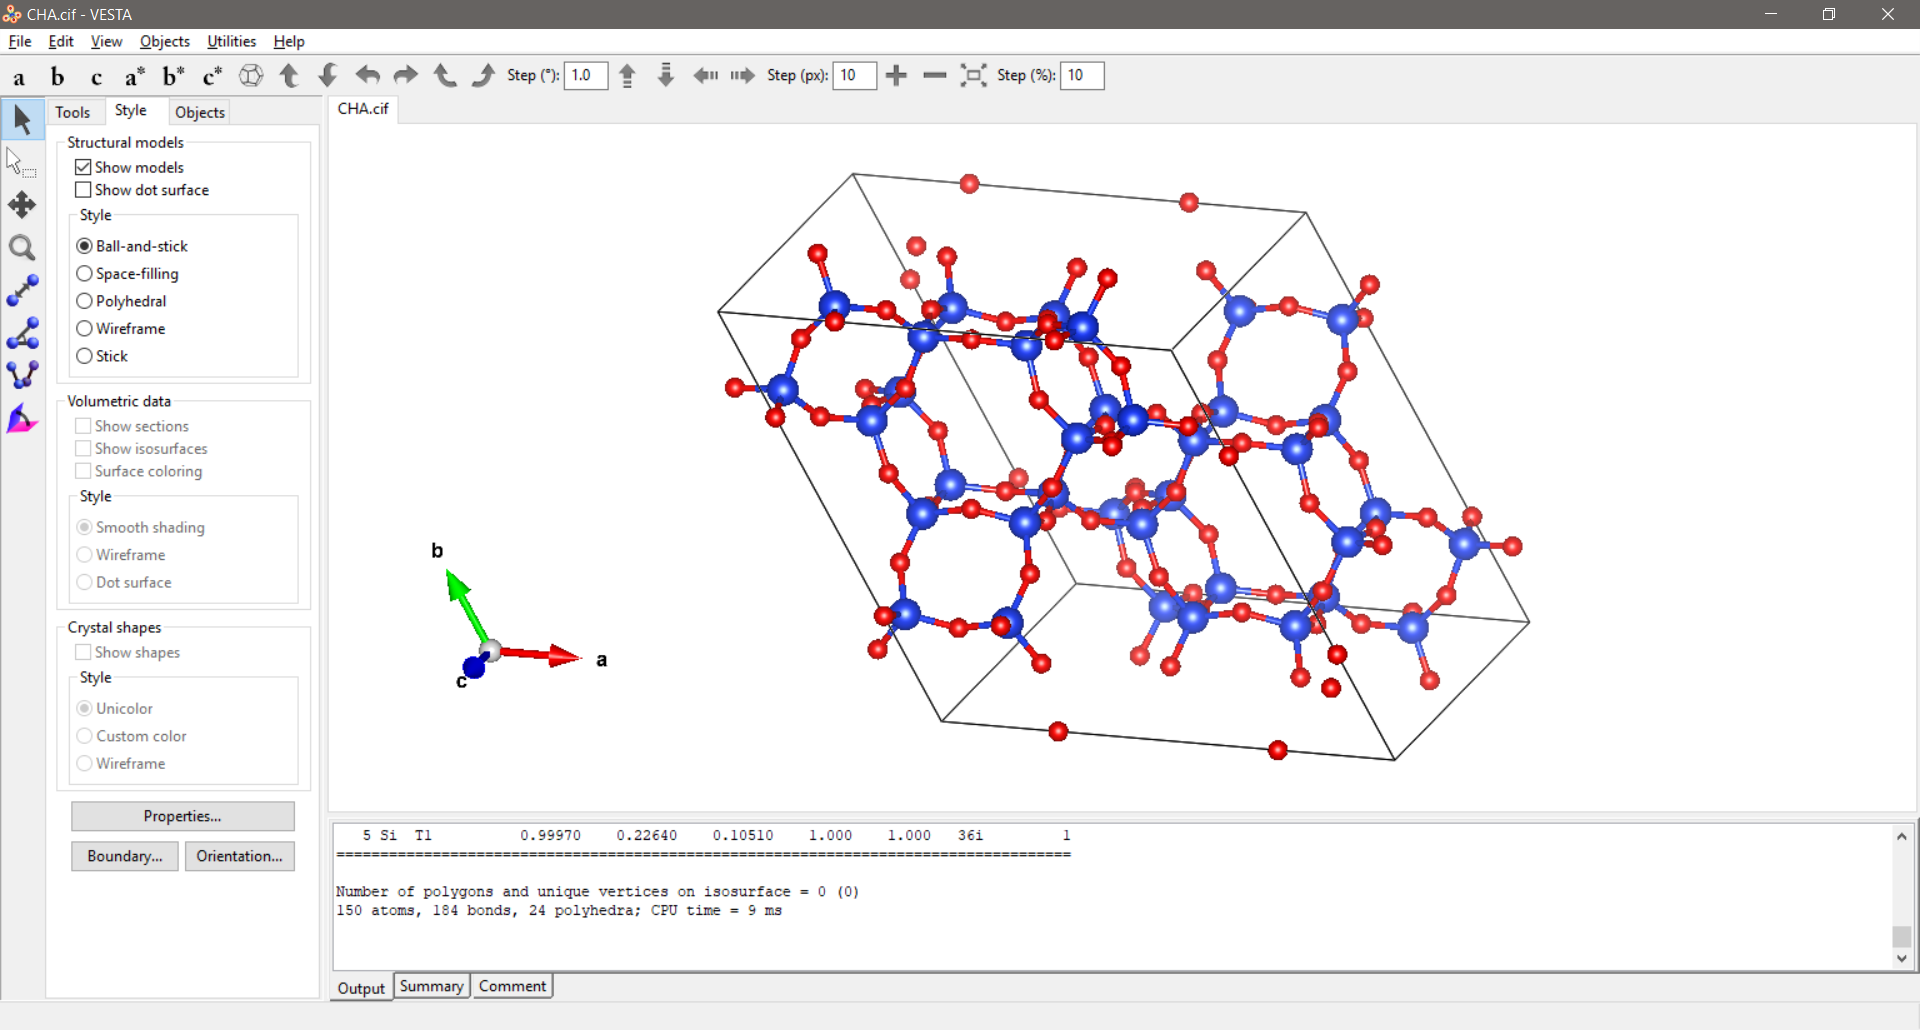
\includegraphics[scale=0.2]{VESTA-UI.png}
\caption{De user interface van VESTA3}
\end{figure}

\par
 Omdat de broncode van VESTA niet openbaar beschikbaar is, is het vrijwel onmogelijk eigen features toe te voegen, en hangt de gebruiker vast aan de tools die deze software ter beschikking stelt. Deze beperking aan vrijheid heeft ertoe geleid dat wetenschappers op zoek gaan naar andere software die dit wel aanbiedt.

\subsection{Andere 3D visualisatiesoftware}
Naast VESTA bestaat er nog een groot aanbod aan andere software die in staat zijn kristallen driedimensionaal te visualiseren. Het Crystalmaker softwarepakket biedt het programma Crystalviewer, Figuur[2.6], gratis aan voor persoonlijk gebruik. Het strak design en de gebruiksvriendelijke user interface geven de software een luxueus gevoel. Voor het gebruik van het volledig potentieel van dit programma en om toegang te krijgen tot de documentatie wordt de gebruiker ertoe gedwongen het eerder dure, volledige softwarepakket aan te kopen. Hiernaast biedt de gratis versie niet de mogelijkheid andere formaten in te lezen dan het .crystal – formaat, wat niet gezien wordt als standaardformaat en niet bestaat in de kristallografische databanken. 

\begin{figure}[h]
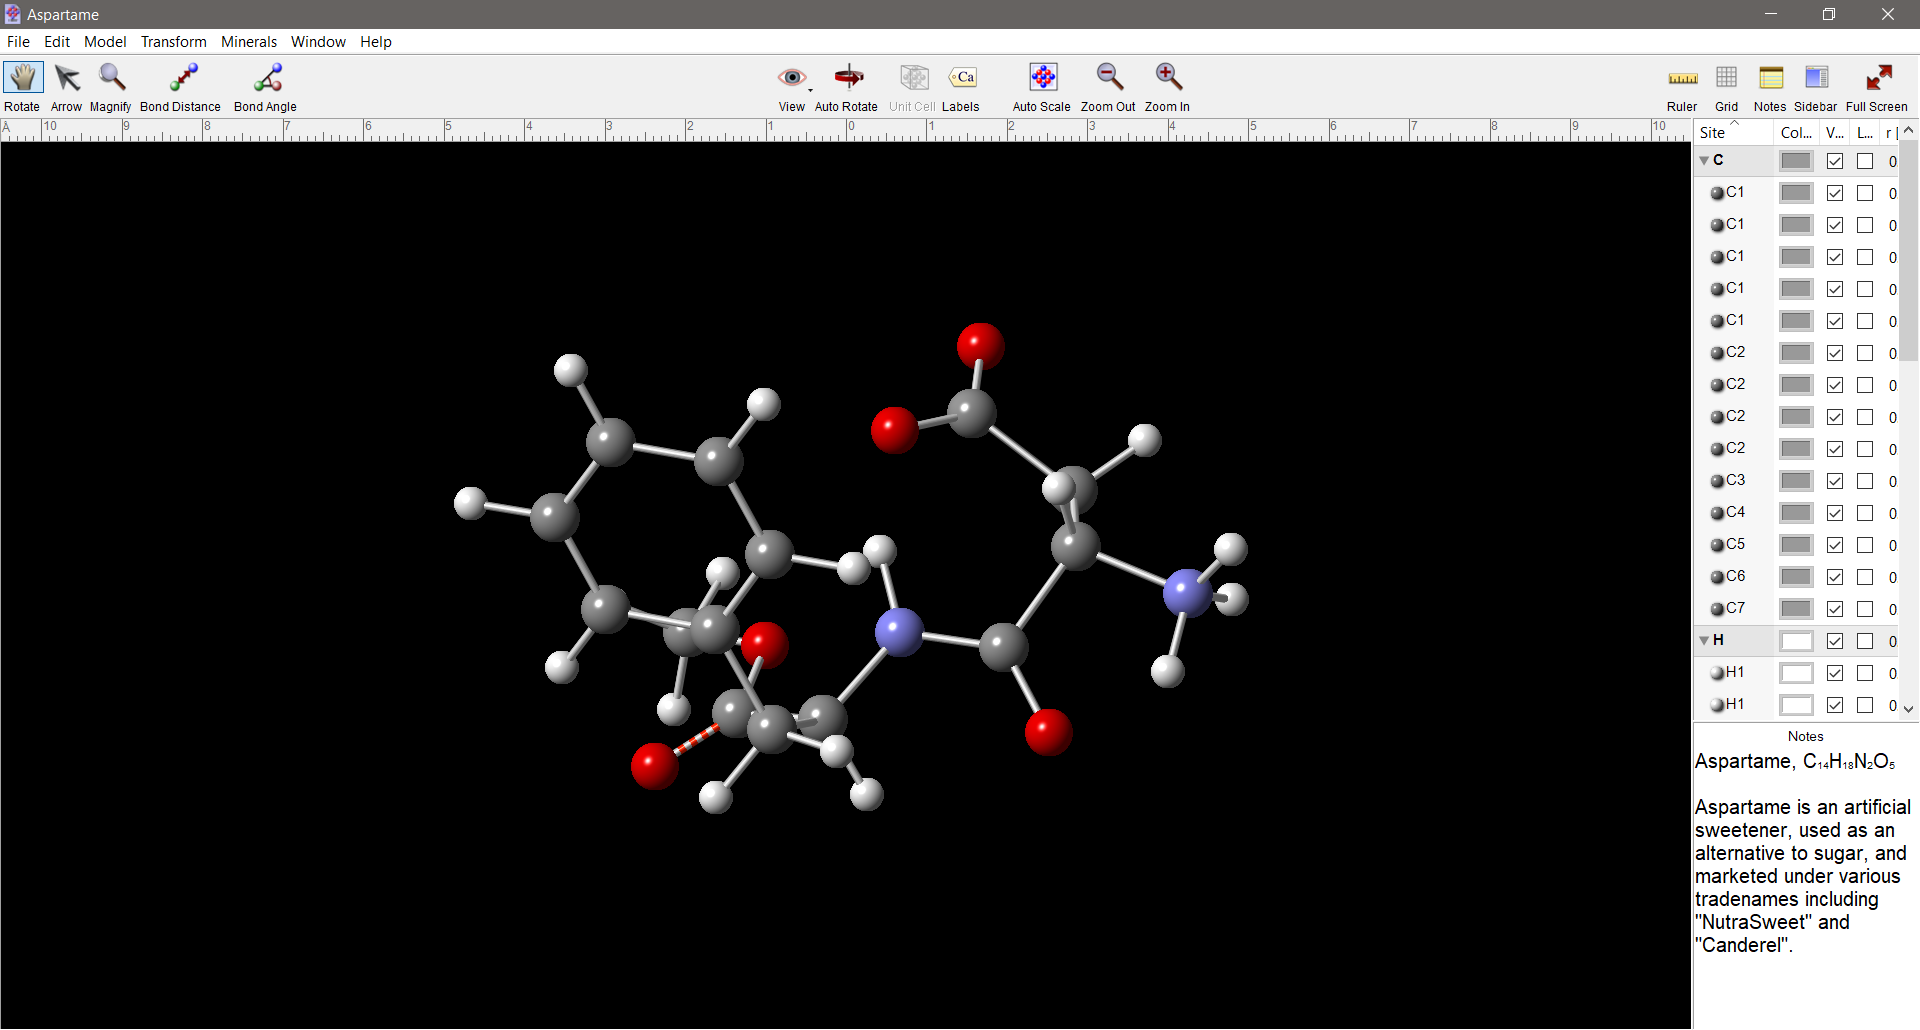
\includegraphics[scale=0.2]{Crystalviewer9-UI.png}
\caption{De user interface van Crystalviewer9}
\end{figure}

\par
Een andere bekende tegenhanger van VESTA is Olex\textsuperscript{2}, zie Figuur[2.7]. Olex\textsuperscript{2} biedt, net zoals VESTA, een groot aantal features aan, welke duidelijk beschreven worden in een overzichtelijke documentatie. Het softwarepakket is volledig gratis en ter beschikking van iedereen. Olex\textsuperscript{2} is volledig geschreven in Python en maakt gebruik van enkele bibliotheken die de gebruiker de mogelijkheid biedt verschillende kristalbeschrijvingsformaten, waaronder CIF, in te lezen en te visualiseren. Ondanks de features en documentatie is het gebruiken van Olex\textsuperscript{2} minder eenvoudig dan de eerder geziene programma’s. Bij het testen van dit programma trad er ook een probleem op bij het visualiseren van een CIF-bestand, wat deze software voor deze toepassing vrijwel onbruikbaar maakt.

\begin{figure}[h]
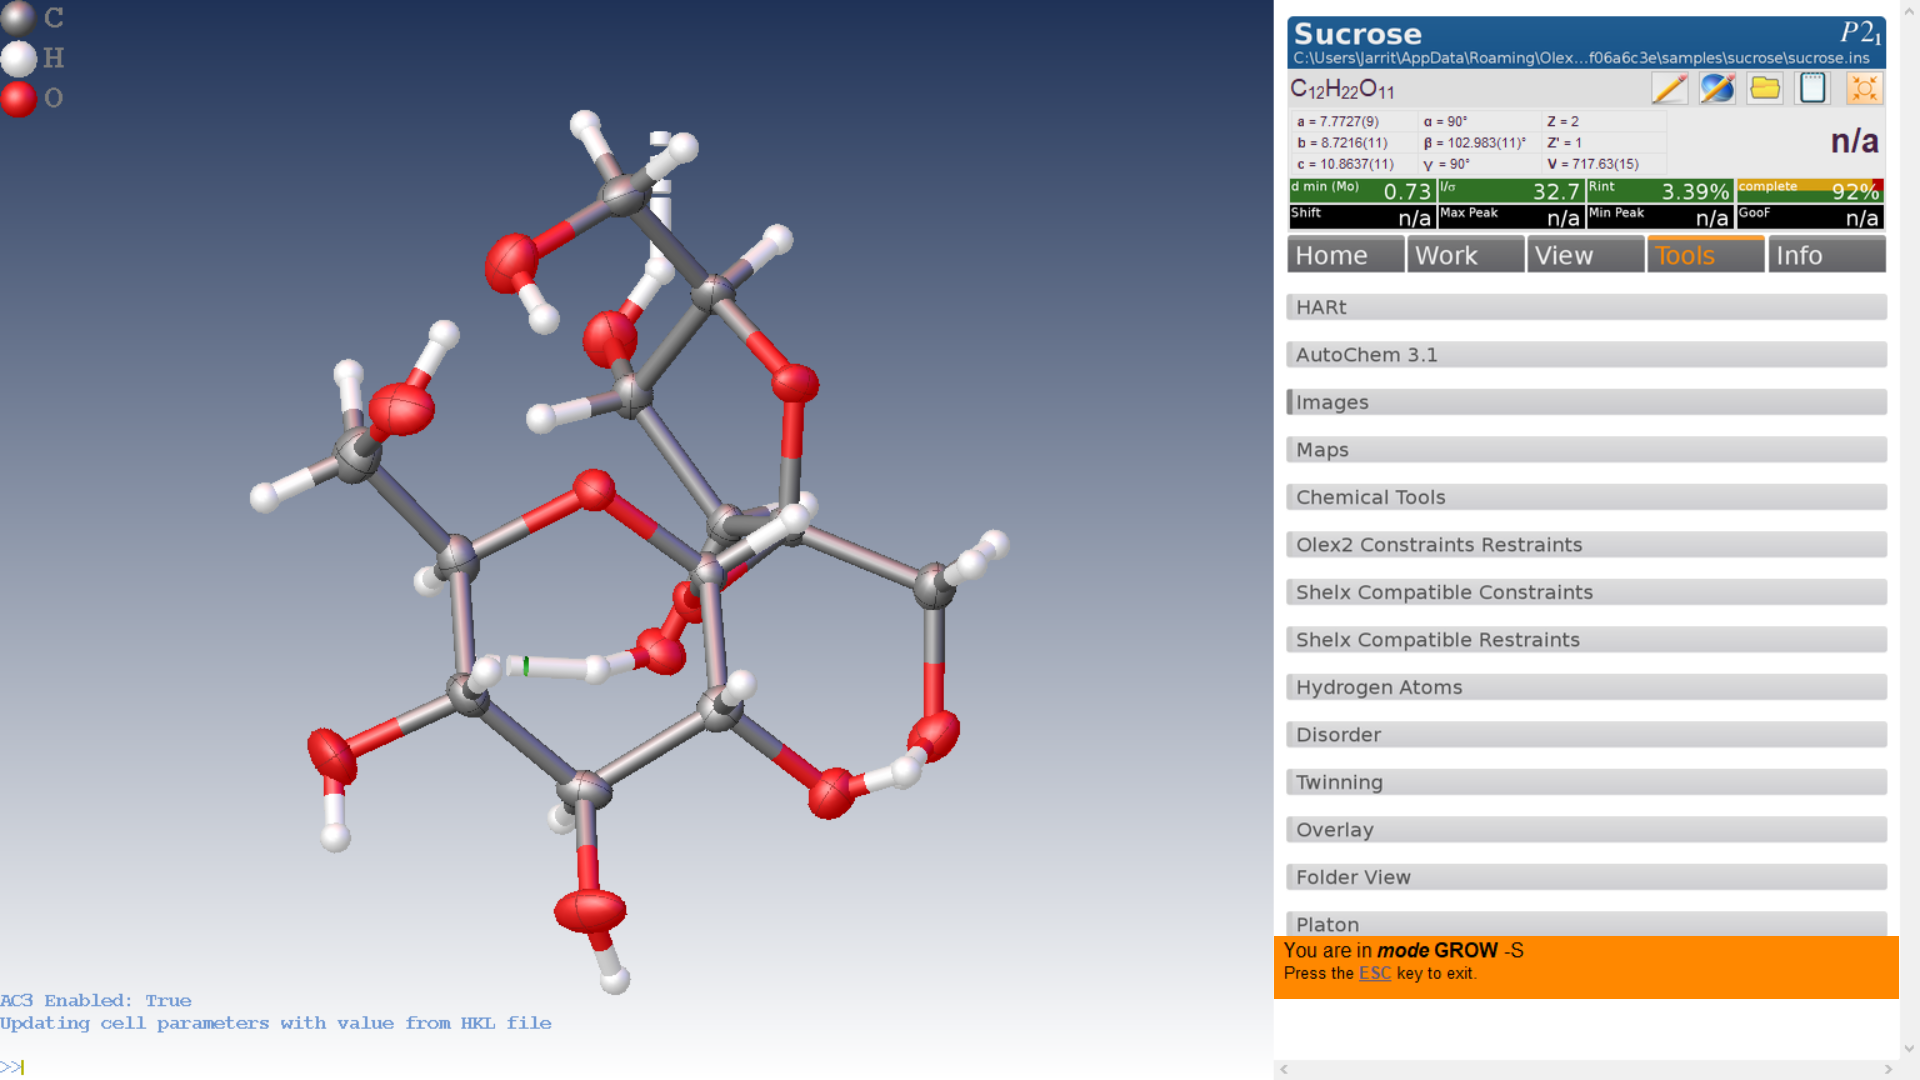
\includegraphics[scale=0.2]{Olex2-UI.png}
\caption{De user interface van Olex\textsuperscript{2}}
\end{figure}

\section{CIF-Parsers}
\subsection{Wat is een parser}
Een parser wordt gezien als een computerprogramma of script dat in staat is een input om te zetten naar een datastructuur met als voorwaarden dat deze input volgens een bepaalde structuur, denk XML, is ingegeven. De parser gaat in de ingevoerde gegevens op zoek naar herkenbare elementen en slaat deze op volgens een eerder genoemde datastructuur, bijvoorbeeld een boomstructuur of een dictionary. Sommige parsers worden gebruikt om ingegeven data te visualiseren, deze data kan dan worden gevisualiseerd in de vorm van een boomstructuur of een grafiek. Een ander soort van parsers heeft als nut de gegevens van het bestand om te zetten in een dictionary, waardoor deze in een ander programma eenvoudig kunnen worden opgevraagd. In dit onderzoek is er nood aan dit tweede type van parser, zodat de gegevens in een CIF-bestand kunnen worden omgezet naar door de module leesbare data. 

\par
\subsection{Het schrijven van een parser}
Om een parser te schrijven voor een bepaald bestandstype of formaat is er eerst een goede kennis nodig van dit formaat. Hoewel het op eerste zicht misschien niet logisch lijkt, wordt het schrijven van een parser eenvoudiger naarmate de striktheid van het formaat stijgt. Er moet minder rekening worden gehouden met alle mogelijke variaties die in het bestand kunnen voorkomen. Zoals in sectie twee besproken werd, bestaan er in het CIF-formaat weinig regels op vlak van tekststructuur. Hierdoor vergt het schrijven van een CIF-parser veel werk. In dit onderzoek is er aanvankelijk geprobeerd een eigen parser te ontwerpen die kan gebruikt worden om CIF-bestanden om te zetten naar bruikbare data. Dit proces wordt in hoofdstuk drie in meer detail besproken. Omdat dit echter niet het doel is van dit onderzoek, is er besloten te kijken naar de mogelijkheden die reeds bestaande CIF-parsers kunnen bieden. De bekeken parsers worden verder beschreven.  

\par
\subsection{The Computational Crystallography Toolbox (cctbx)}
Dit project heeft als voornaamste doel een brug te bouwen tussen kristallografische data en het gebruik hiervan in computer gerelateerde toepassingen. Het project is volledig open source, wat wil zeggen dat het volledig toegankelijk en gratis is voor iedereen die het wil gebruiken, hiernaast zorgt dit ervoor dat dit project voortdurend wordt verbeterd en stijgt in functionaliteit. Deze toolbox ligt ook aan de basis van de visualisatiesoftware Olex\textsuperscript{2}, welke beschreven wordt in de derde sectie van dit hoofdstuk. De grote omvang van dit project en het grote aantal functionaliteiten maakt het, ondanks de duidelijke documentatie, ook meer ingewikkeld om dit te gebruiken. 

\subsection{Python CIF Read/Write (PyCIFRW)}
Naast het inlezen van CIF-bestanden kunnen deze bestanden met dit programma ook gecreëerd en aangepast worden. Ook dit programma is open source, omdat dit op een kleinere schaal gebeurt dan cctbx, zie vorige, zijn de mogelijkheden, hoewel meer beperkt, geschikter voor gebruik in dit onderzoek. Door de goede documentatie van dit project en de volledige ondersteuning van Python kan dit programma gecombineerd worden met de, in de volgende sectie besproken, Blender API. \citep*{PYCIFRW1} Voor deze thesis is de schrijffunctie minder van belang, deze zal niet worden bekeken. 

\lstset{caption = Werken met PyCIFRW in Python3}
\lstinputlisting{listings/parservb.py}

\par 
Listing[2.7] is een voorbeeld van hoe PyCIFRW kan worden gebruikt in Python om een CIF-file in te lezen. De voornaamste functies worden hier weergegeven. Een meer gedetailleerde beschrijving van de werking van PyCIFRW kan worden teruggevonden in hoofdstuk 4.

\section{Blender en de Blender API}

\subsection{Gratis software}
Blender beschrijft zichzelf als een \enquote{open-sourced, community development program}, en is het collectieve werk van softwareontwikkelaars overal ter wereld. \citep*{BLEN1} De ontwikkeling en het correct functioneren van dit programma wordt overzien door The Blender Foundation, een Nederlandse, onafhankelijke, non-profit stichting. Dit alles leidt ertoe dat de Blender software gratis verkrijgbaar is voor iedereen die het wenst te gebruiken.

\subsection{Blender in de bedrijfswereld}
Zoals in het verdere verloop van deze sectie duidelijk zal worden, heeft Blender een groot aantal verschillende toepassingen. Hierdoor wordt Blender niet enkel door amateurs gebruikt, maar ook door bedrijven in verschillende industrieën waaronder verkoop, manufacturing, game development en vele anderen. Een voorbeeld van de kracht van Blender is Tangent Animation, een animatiestudio die uitsluiten werkt met Blender. In 2018 ontwikkelde dit bedrijf de animatiefilm Next Gen welke te zien is op onder andere Netflix, Figuur[2.8].
\par

\begin{figure}[H]
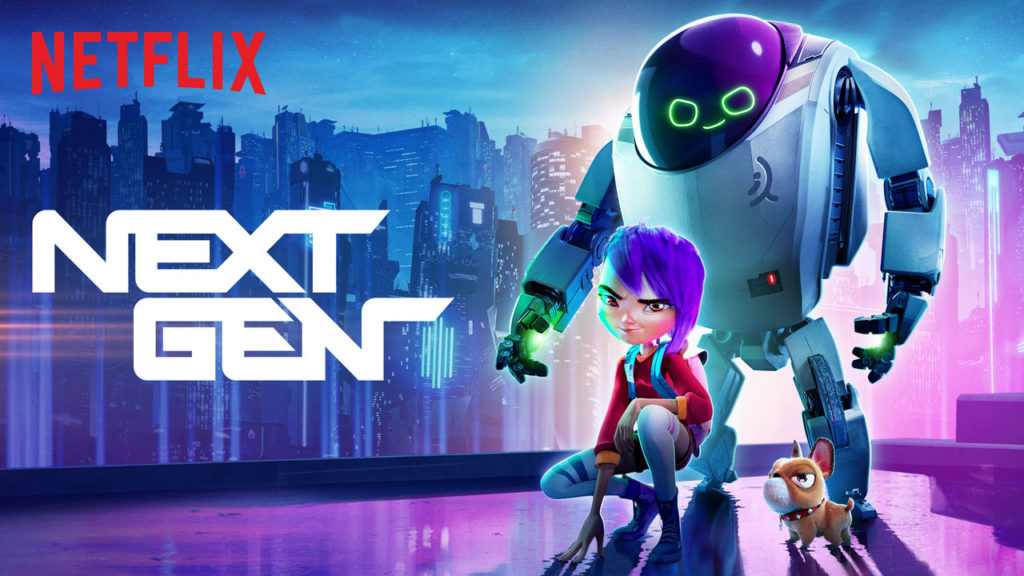
\includegraphics[width=\textwidth,keepaspectratio]{next-gen-poster.png}
\caption{Poster van de film Next Gen \citep*{NEXT1}}
\end{figure}

    



\subsection{De Blender interface}
Na het opstarten van Blender wordt de gebruiker begroet met de Blender interface. Een niet ervaren gebruiker zal, naast onder de indruk, vooral in de war zijn en niet weten waar te beginnen. In Figuur[2.9] wordt het startscherm weergegeven en worden enkele onderdelen ervan beschreven. Veel van deze tools en hoe deze werken vallen niet binnen het bestek van deze tekst en worden weinig of niet uitgelegd, hiervoor wordt verwezen naar online handleidingen en de documenten waar deze tekst op gebaseerd is.\citep*{BLEN1}\citep*{API1} 

\begin{figure}[h]
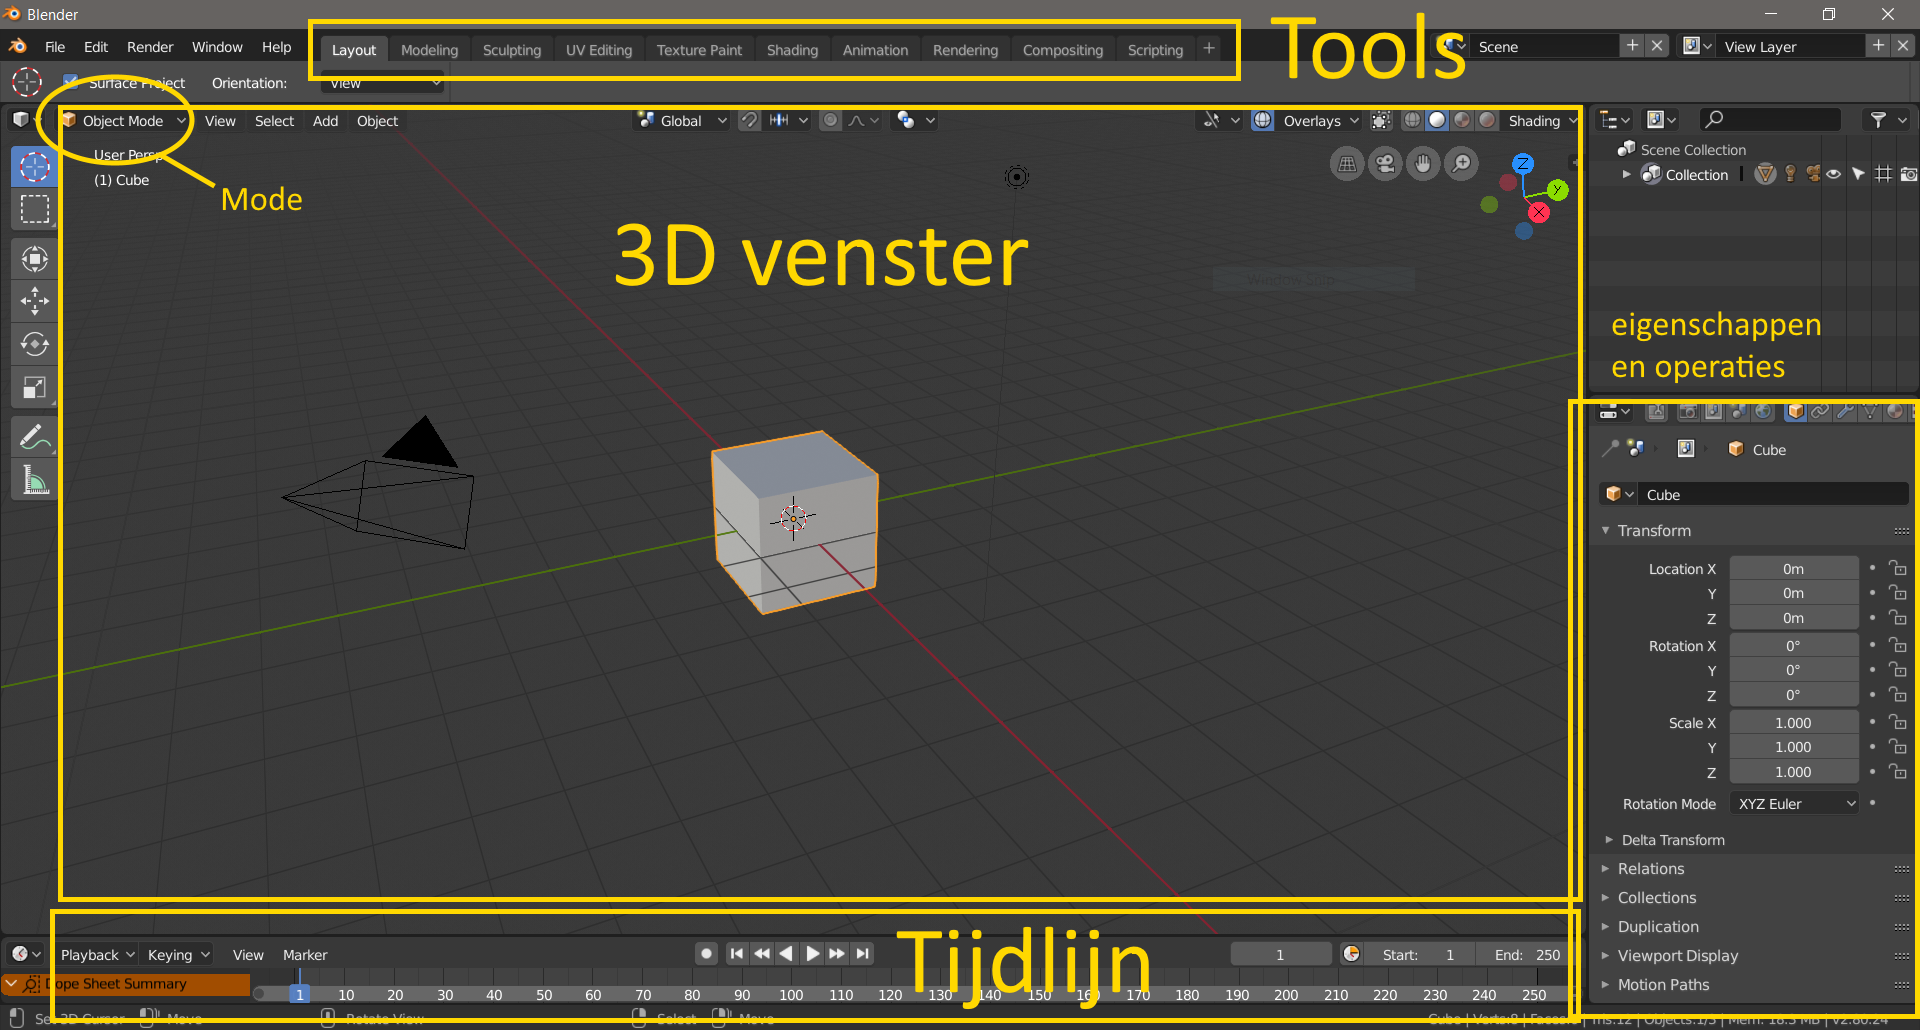
\includegraphics[scale=0.3]{Blender.png}
\caption{Het Blender startscherm}
\end{figure}

\par
In het midden van het scherm kan het 3D venster worden teruggevonden. Hier worden alle objecten weergegeven die zich op de huidige ingeschakelde layers bevinden. Het gebruik van layers laat toe objecten op een andere layer tijdelijk te verbergen om zo een duidelijk overzicht te behouden over het huidige werk. Wanneer een object wordt aangemaakt zal deze automatisch geplaatst worden op de huidige layer. De Blender interface heeft twee modes: object mode en edit mode.
\\
In object mode kan een object in zijn geheel bewerkt worden. Transleren, roteren en herschalen zijn slechts enkele van het groot aantal objectoperaties dat Blender aanbiedt. 
\\
Edit mode laat de gebruiker onder andere toe de vorm van het object aan te passen door hoekpunten aan te duiden en te verplaatsen. 
Objecten toevoegen wordt gedaan met de Add knop linksboven in het venster. 
In Blender gebruikt men de rechtermuisknop om items te selecteren en te verplaatsen. Het klikken op de linkermuisknop verplaatst de 3D cursor, dit is de plaats waar nieuwe objecten terechtkomen wanneer ze worden aangemaakt. Ten slotte kan in het 3D venster worden bewogen door het indrukken van het muiswiel.

\par
Met deze informatie kan er een object aangemaakt en verplaatst worden en kunnen er enkele basisoperaties op worden toegepast. Dit is voorlopig alles wat er over het bewerken van objecten gezegd zal worden. Dit is slechts het topje van de enorme ijsberg die Blender wordt genoemd.


\subsection{Kleuren, texturen en materialen}
Blender laat de gebruiker toe de gemaakte objecten, naast vorm, ook kleur te geven. Eerst krijgt het object een materiaal toegekend, waarna de eigenschappen van dit materiaal kunnen worden aangepast. Deze eigenschappen zijn onder andere de kleur, lichtuitstraling, weerspiegeling, schaduw en doorzichtigheid van het object. Om het object er nog realistischer te laten uitzien kan er een textuur op het object worden gezet. Deze geven het object een bepaalde oppervlaktestructuur of uiterlijk. Blender voorziet een aantal basistexturen maar de gebruiker kan zelf afbeeldingen gebruiken om het voorwerp een textuur te geven. Wanneer de objecten een kleur of textuur hebben kan de gebruiker deze renderen. Dit gaat alle lichtinteracties en schaduws berekenen, wat erg computerintensief kan zijn. In Figuur[2.10] wordt de uitkomst van het renderen van een Blender project weergegeven, door slim gebruik van texturen en materiaaleigenschappen was de ontwerper in staat een 3D tekening levensecht te laten lijken.\citep*{BLEN2}

\begin{figure}[h]
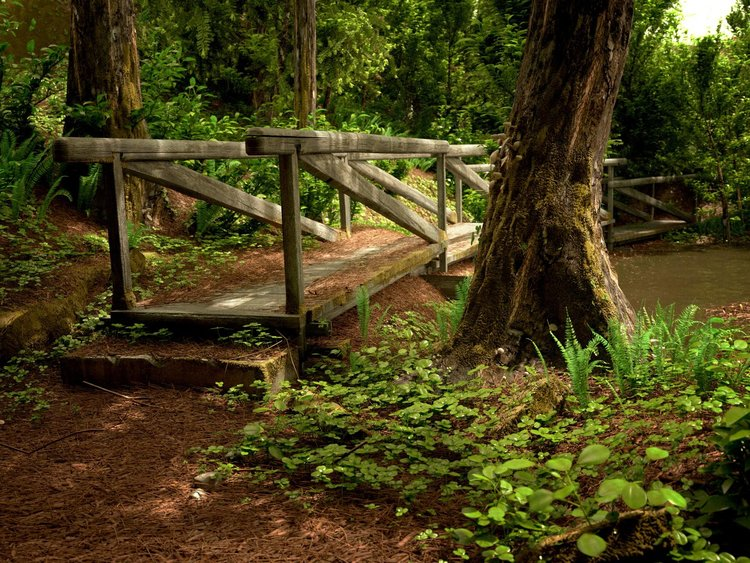
\includegraphics[scale=0.5]{blenderreal.png}
\caption{Het Blender project van de winnaar van een fotorealiteit wedstrijd, na rendering}
\end{figure}

\subsection{Andere opmerkelijke tools in Blender}
Naast het aanmaken, vervormen en inkleuren van objecten biedt Blender nog een handvol extra mogelijkheden aan. Met de Sculpting tool kan men objecten boetseren tot in de kleinste details. Dit kan leiden tot realistische beeldhouwwerken.

\par 
Onderaan de interface afgebeeld op Figuur[2.9] kan het tijdlijn-venster gezien worden. Dit venster behoort tot de animation tool van Blender, door een aantal gerenderde frames snel opeenvolgend achter elkaar te laten afspelen wordt een video verkregen. Kleine verschillen tussen deze frames geven de indruk dat het object beweegt, dit wordt een animatie genoemd. 

\par
Hoewel er betere software bestaat om dit te doen, is het in Blender, door gebruik te maken van scripts, mogelijk volledig functionele 3D videogames te ontwerpen. Zo bestaan er reeds games die volledig in Blender zijn gemaakt en te koop staan op Steam, een bekende videogames-distributeur.

\subsection{Scripten in Blender met de Blender API}
Nog een belangrijke functie die Blender aanbiedt, en in de vorige sectie niet werd vermeld, is de mogelijkheid tot het scripten in Blender zelf, in tegenstelling tot de game-engine. Omdat deze feature in zekere mate de rode draad is van deze thesis, wordt er een volledige subsectie gewijd aan dit eerder ingewikkelde onderdeel van Blender.

\par
In de tweede sectie van dit hoofdstuk werd besproken hoe operaties in Blender kunnen uitgevoerd worden met behulp van de Blender interface. Er bestaat echter een andere manier om operaties uit te voeren, namelijk via scripts. Met de juiste kennis kan er met behulp van scripts zelfs meer gedaan worden dan met enkel de interface. 
Het schrijven van scripts wordt gedaan aan de hand van Python 3, verder gerefereerd als Python. Alle standaardmodules in Python kunnen dan ook gebruikt worden, hiernaast is het mogelijk zelf modules te importen, in het geval van dit onderzoek een CIF-Parser. Aan de hand van de Python logica is het eenvoudig loops te cre\"{e} ren die automatisch een aantal objecten aanmaakt in Blender. Hieronder wordt kort de Blender API beschreven.

\par
De Blender API biedt een aantal modules aan die gebruikt kunnen worden, naast alle reeds bestaande functionaliteiten van Python. De voornaamste van deze modules is de bpy module, die alle functies bevat in verband met het aanmaken en aanpassen van objecten in Blender. De bpy module is zodanig groot dat deze nogmaals wordt opgedeeld in submodules, deze worden samen met hun taak weergegeven in tabel[2.2]. In de documentatie van de Blender API worden alle methodes van deze modules uitgelegd. In hoofdstuk vier wordt dieper ingegaan op het gebruik van de Blender API en de toepassing ervan in dit onderzoek.

\begin{table}[H]
\caption{De submodules van de Blender bpy module \citep*{API1}}
\begin{center}
\begin{tabular}{|c|l|}
\hline
\textbf{bpy.ops}                       & Bevat alle operators voor het maken en aanpassen van objecten       \\ \hline
\textbf{bpy.context}                   & Geeft de mogelijkheid specifieke data op te vragen                  \\ \hline
\textbf{bpy.data}                      & Bevat alle data van de objecten                                     \\ \hline
\textbf{bpy.app}                       & Hulpmodule bij het schrijven van add-ons en extra functionaliteiten \\ \hline
\textbf{bpy.types,bpy.utils,bpy.props} & Hulpmodules bij het schrijven van add-ons                           \\ \hline
\textbf{bpy.path}                      & Vrijwel identiek aan de os.path submodule van Python                \\ \hline
\end{tabular}
\end{center}
\end{table}


\section{Conclusie}

Kristallografie is een speciefieke tak in de wetenschap die zich bezighoudt met het onderzoeken van kristallen, hun structuur en hun eigenschappen. Een kristal wordt opgebouwd uit eenheidscellen. Het beschrijven van zo'n eenheidscel geeft alle informatie van het kristal. De vorm van een eenheidscel wordt bepaald door zes roosterparameters en een van de 14 Bravaisroosters. Deeltjes kunnen zich op 240 manieren in de eenheidscel bevinden, de ruimtegroepen genaamd.
\par
In het CIF formaat is alle informatie over een kristalstructuur terug te vinden, het is leesbaar door zowel computers als mensen. CIF bestanden worden geschreven in ASCII wat eenvoudige leesbaarheid en aanpasbaarheid toelaten. Gebaseerd op het STAR formaat heeft het CIF formaat enkele syntactische restricties waaraan moet gehouden worden. De structuur van CIF bevat datablokken, data-elementen en lussen om de data weer te geven.
\par
De bestaande 3D kristalvisualisatiesoftwarepakketten zijn vaak moeilijk in omgang, duur of bieden niet genoeg vrijheid. VESTA en Olex\textsuperscript{2} zijn gratis programma\'{}s die kristalstructuren kunnen visualiseren en geven de gebruiker een aantal handige tools om onderzoek te vereenvoudigen. Ze hebben echter hun nadelen wat leidt tot de vraag naar andere programma's.
\par
Parsers hebben als functie data te extraheren uit bestanden met een bepaalde syntax. Ze worden gebruikt om data te visualiseren of bruikbaar te maken in andere toepassingen. De complexiteit van het schrijven van een parser is omgekeerd evenredig met het aantal syntaxregels van een formaat, hierdoor is het schrijven van een CIF parser eerder moeilijk. Cctbx en PyCIFRW zijn open source modules die in staat zijn CIF bestanden te parsen.
\par
Blender is een gratis, open source project waarin driedimensionale tekeningen kunnen worden gemaakt. Met een groot aantal tools, waaronder animeren, sculpten en een eigen game-engine, geeft Blender de gebruiker veel vrijheid en mogelijke toepassingen. Door gebruik te maken van texturen en materialen kunnen er fotorealistische tekeningen gemaakt worden. Scripten in Blender laat het automatiseren van tekenen toe en wordt gedaan aan de hand van Python scripts en de modules uit de Blender API.   
%%%%%%%%%%%%%%%%%%%%%%%%%%%%%%%%%%%%%%%%%%%%%%%%%%%%%%%%%%%%%%%%%%% 
%                                                                 %
%                           INLEIDING                             %
%                                                                 %
%%%%%%%%%%%%%%%%%%%%%%%%%%%%%%%%%%%%%%%%%%%%%%%%%%%%%%%%%%%%%%%%%%% 


\chapter{Ontwerpproces}

In dit hoofdstuk worden de ondernomen stappen besproken bij het ontwerpen van een interface die kristalstructuren, in de vorm van een CIF-bestand, kan visualiseren in Blender. Dit hoofdstuk is met opzet kort en relatief oppervlakkig gebleven zodat de lezer de werking van het programma op een overzichtelijke manier kan doornemen. Een meer gedetailleerde beschrijving van dit proces kan worden gevonden in hoofdstuk vier, hier wordt ook dieper ingegaan op de installatie van de twee externe programma's, OpenBabel en PyCIFRW, die zullen besproken worden in dit hoofdstuk.
\par
De eerste sectie beschrijft hoe de inwendige symmetrie een probleem vormt bij het visualiseren van kristallen, wat het programma OpenBabel doet en hoe het gebruiken hiervan een oplossing biedt op dit probleem.
In de tweede sectie zullen de datastructuren worden uitgelegd die worden gebruikt, hoe, met behulp van een parser, een CIF-bestand kan worden omgezet in verwerkbare data en ten slotte  hoe de verkregen kristaldata zal worden opgeslagen in deze datastructuren.
Het visualiseren van de kristaldata in Blender zal worden besproken in sectie drie. In deze sectie zal worden uitgelegd hoe de omkadering van het eenheidskristal, de atomen en hun onderlinge bindingen worden getekend.
De vijfde sectie beschrijft wat er komt kijken bij de creatie van een add-on in Blender. 
In de laatste sectie wordt een conclusie getrokken over de onderwerpen die in dit hoofdstuk worden besproken.


\section{Omvormen van het invoersbestand}

\subsection{Symmetrieoperaties in het CIF-formaat}
Zoals in sectie 2.1.5 van deze tekst staat beschreven kan een kristal worden beschreven aan de hand van een aantal parameters en een lijst van elementen. Dit kan ook gezien worden in het CIF-bestand van Chaziet[Bijlage B] waar slechts vijf atomen worden beschreven terwijl het eenheidskristal in het totaal uit 150 atomen bestaat. Dit is erg handig aangezien er dertig keer zo weinig atomen moeten worden beschreven. In dit onderzoek vormt dit echter een probleem. Om een kristal te tekenen dient natuurlijk de positie van elk element gekend te zijn.
\par
Aan de hand van de ruimtegroep en de centering van het kristalrooster kunnen alle symmetrieoperaties worden verkregen. Deze symmetrieoperaties zijn in het CIF-formaat reeds gegeven in het blok \textit{\_symmetry\_equiv\_pos\_as\_xyz} als een lijst van fractionele coördinaten. Vanuit deze symmetrieoperaties kunnen de posities van elk element in het kristal berekend worden. Er dient rekening gehouden te worden met de mogelijkheid dat één bepaald element aan de hand van verschillende berekeningen kan verkregen worden zodat dit niet meermaals wordt genoteerd, en later getekend. Het is mogelijk een functie te schrijven die de lijst van symmetrieoperaties ophaalt en vervolgens voor elk van deze symmetrieoperaties de positie van de elementen berekenen die ze representeren. Er bestaan echter reeds programma's die dit soort berekeningen kunnen doen, OpenBabel is hier één van.
\par
\subsection{OpenBabel}
OpenBabel is een open source chemische toolbox die gebruikt wordt om chemische data te zoeken, analyseren en te converteren.\citep*{OBAB1} Naast het converteren tussen een groot aantal chemische dataformaten kan OpenBabel ook binnen eenzelfde formaat data converteren. Deze functionaliteit laat onder andere toe de kristaldata van een CIF-bestand om te zetten naar data van datzelfde kristal met een andere ruimtegroep. Door de ruimtegroep aan te passen naar dat van P 1, een vorm van P centrering waarbij er geen inwendige symmetrie bestaat, zal elk element dat beschreven wordt slechts op één plaats voorkomen in het kristal. In plaats van een lange lijst van symmetrieoperaties zal elk element dat gevormd kan worden door deze operaties in het blok met de atoombeschrijvingen komen te staan.   
\par
De broncode van OpenBabel staat vrij beschikbaar op hun GitHub pagina.  Hiernaast is het ook mogelijk de GUI-versie van OpenBabel te downloaden door de installatie-instructies te volgen die te vinden zijn op hun officiële webpagina.\citep*{OBAB1}   
\par
\begin{figure}[h]
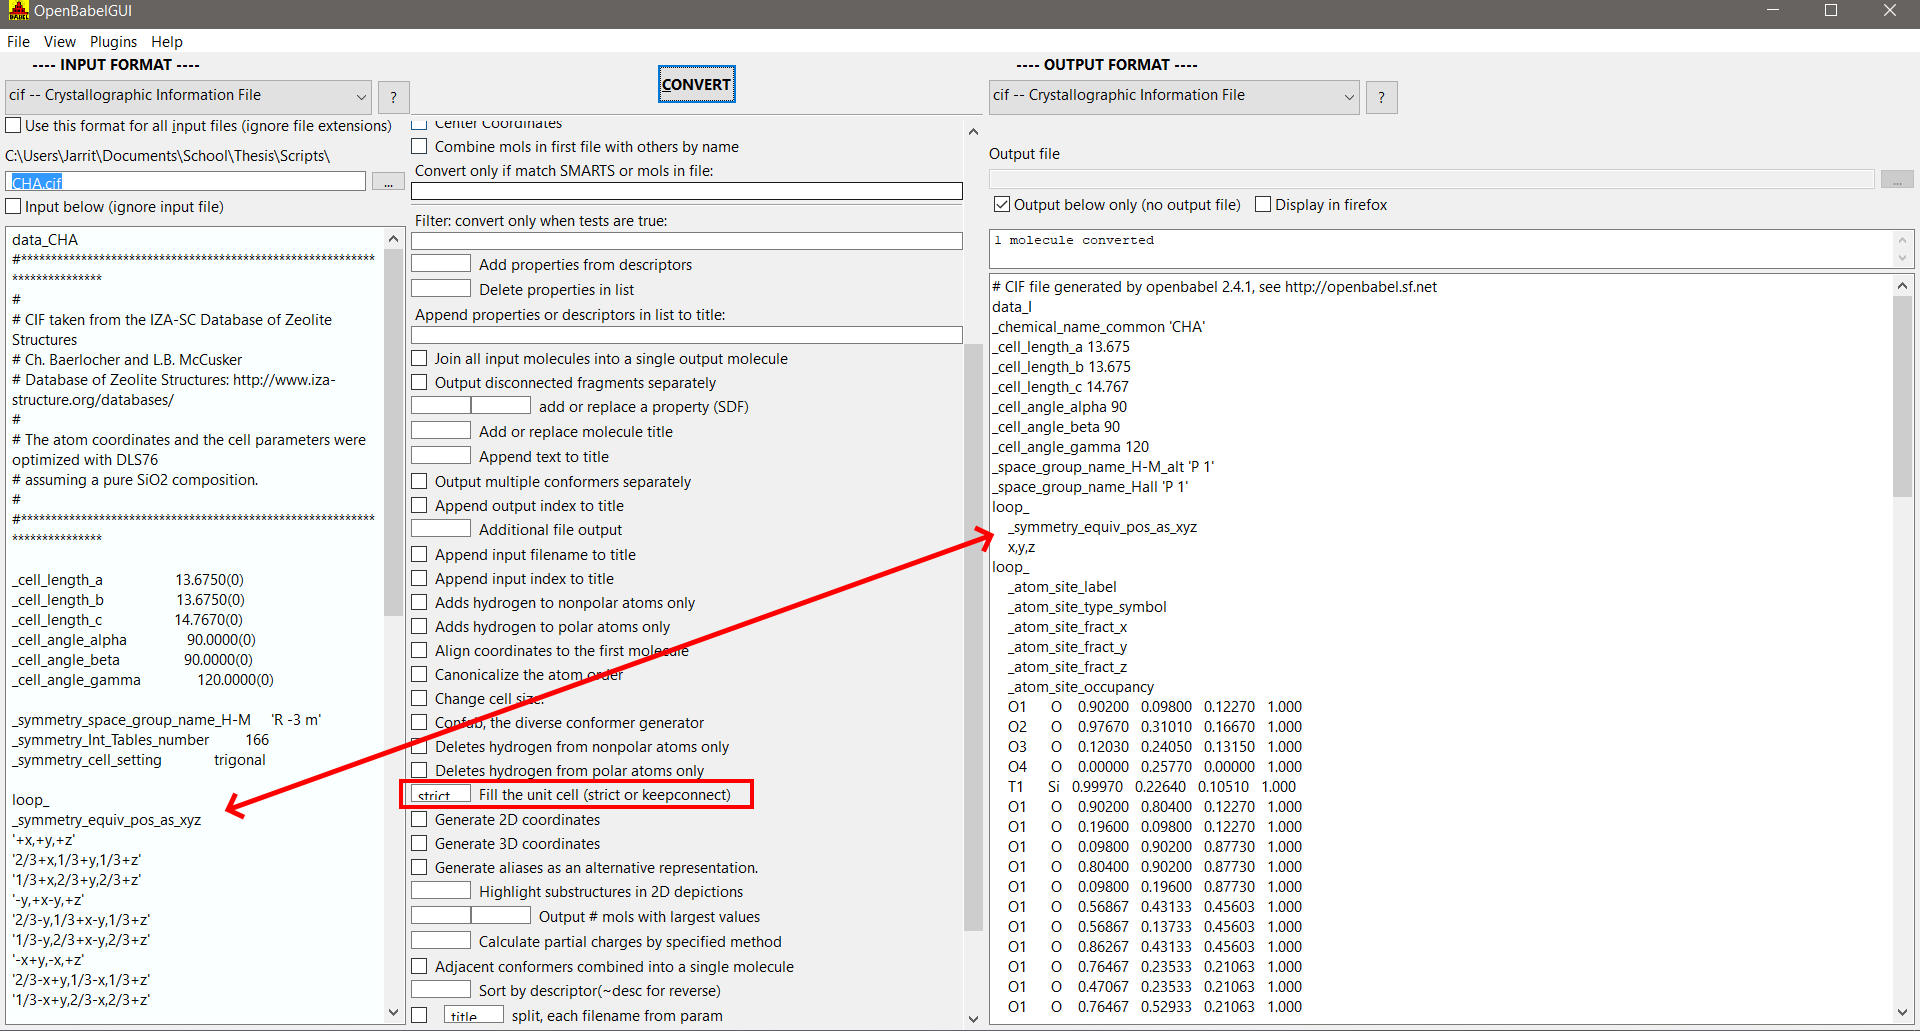
\includegraphics[width=\textwidth,keepaspectratio]{OpenBabelGUI.png}
\caption{Conversie van ruimtegroep met OpenBabel GUI}
\end{figure}
\par
In figuur[3.1] wordt de GUI van OpenBabel afgebeeld. In de linker- en rechterkolom van dit venster staan de in- en uitvoer van het programma en hun formaat. In de middelste kolom kunnen verschillende soorten van conversies worden aangeduid. In het geval van de afbeelding zijn zowel in- als uitvoer in het CIF-formaat en staat het \textit{Fill the unit cel}-vakje op \textit{strict}. Deze opties zorgen ervoor dat het invoerbestand zal worden omgezet naar een ander CIF-bestand maar ditmaal zonder symmetrieoperaties, wat duidelijk wordt bij het bekijken van de twee buitenste kolommen. Bij dit voorbeeld is er maar een optie aangeduid, er zijn nog een groot aantal erg handige keuzemogelijkheden maar deze komen voorlopig niet aan bod.
\par
Hoewel de OpenBabel GUI het converteren van data erg eenvoudig en overzichtelijk maakt, zou het niet erg efficiënt zijn dat dit proces manueel moet worden gedaan voor elk kristal. Deze software kan echter ook vanuit een terminal worden uitgevoerd, wat, in combinatie met de subprocess module van python, de kristallografische interface toelaat deze conversie automatisch te laten verlopen. In hoofdstuk vijf wordt dit in meer detail uitgelegd.
\par     
\section{Van CIF naar py}

\subsection{Ontwerpen van datastructuren}
Nu het CIF-bestand naar een meer bruikbaar formaat is omgezet, is er nood aan datastructuren waarin de informatie kan geparsed worden. Zo een datastructuur noemt men een klasse en het werken hiermee wordt object georiënteerd programmeren genoemd. Enkele voordelen dat dit biedt over de klassieke, imperatieve methode van programmeren, zijn overzichtelijkheid, herbruikbaarheid van klassen en een extra laag van veiligheid doordat de data niet rechtstreeks kan worden aangepast.
\par
Het inlezen van de data wordt in drie klassen gedaan. Een eerste klasse, \textit{Cell}, die informatie bevat over het kristalrooster, waaronder de roosterparameters. Deze data-elementen worden ook wel de attributen van een klasse genoemd. Een tweede klasse, \textit{Atom}, die de fractionele coördinaten van het atoom bevat en welk element het voorstelt. De derde klasse, \textit{Crysdata}, overkoepelt voorgaande klassen in de zin dat deze naast de naam van het kristal ook één object van de klasse \textit{Cell} en een lijst van objecten van de klasse \textit{Atom} bevat. Hiernaast bezit elke klasse ook de methode, \textit{printout()}, die de data van de klasse op een nette manier weergeeft op de terminal, en de methode \textit{draw()} die later gebruikt wordt om het object te tekenen in Blender. Methodes zijn functies die op een object van een klasse kunnen worden opgeroepen.  In Figuur[3.2] worden de onderlinge verhoudingen van deze klassen verduidelijkt, dergelijke figuur wordt een klassendiagramma genoemd, en geeft de algemene opbouw van een programma aan de hand van de gebruikte attributen, methodes, modules en hun onderlinge relaties. Uit dit diagram kan er geïnterpreteerd worden hoe de data uit het CIF-bestand met behulp van de PyCIFRW-parser zal worden ingelezen in de drie eerder genoemde klassen.

\begin{figure}[h]
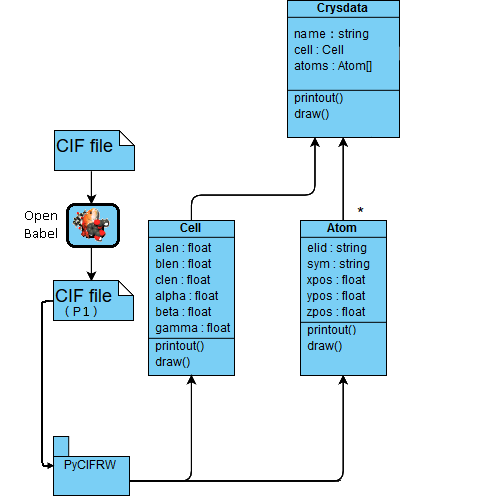
\includegraphics[scale=0.7]{ClassDiagramEz.png}
\caption{Vereenvoudigd klassendiagramma van het programma}
\end{figure}

\subsection{Inlezen van CIF-bestanden}
In de vierde sectie van hoofdstuk twee van deze tekst wordt het nut en de werking van een parser besproken. Er wordt ook gekeken naar twee bestaande programma's die in staat zijn CIF-bestanden te parsen en waarom PyCIFRW de voorkeur krijgt in dit onderzoek.
\par
Door de module \textit{CifFile} te importeren kunnen de schrijf- en leesfuncties van PyCIFRW worden opgeroepen in het programma. Nu kan het bestand, dat eerder werd omgezet met behulp van OpenBabel, worden geparsed. De geparsede data zal in de vorm van een soort dictionary ter beschikking zijn. Een dictionary is een python structuur die bestaat uit een lijst van sleutels, \textit{keys}, en hun corresponderende waarden, \textit{values} genoemd. De data kan verkregen worden door de dictionary op te roepen met een bepaalde sleutel.
\par
De sleutels van de dictionary die de PyCIFRW parser aanmaakt stemmen overeen met de namen die te vinden zijn in het CIF-bestand zelf. Op deze manier kan de data dus bekomen worden die vervolgens in de klassen worden ingevuld.

\section{Tekenen in Blender}
\subsection{Berekenen van de conversiematrix}
Voor er kan getekend worden dienen alle fractionele coördinaten omgezet te worden  naar hun overeenkomstige orthogonale waarden. Dit wordt gedaan aan de hand van een functie die de conversiematrix berekend op de methode die beschreven wordt in de eerste sectie van hoofdstuk twee. Deze matrix wordt opgeroepen wanneer de conversie tussen fractioneel en orthogonaal moet gebeuren.

\subsection{Omkadering van de eenheidscel}
Het eerste en meest eenvoudige object dat getekend wordt zijn de randen van de eenheidscel. Deze acht ribben worden in feite reeds beschreven door de roosterparameters van het kristal. Het tekenen van deze wordt gedaan door de coördinaten van de hoekpunten te berekenen, en tussen elk hoekpunt en zijn drie 'buren' een ribbe te tekenen. Zo een ribbe wordt getekend als een cilinder aangezien lijnen geen volume bezitten en niet als vormen beschouwd worden in Blender. 
\par
Voor het berekenen van de hoekpunten is er niet echt nood aan de conversiematrix. Deze kunnen op een goniometrische manier berekend worden met behulp van de lengte van de ribben en hun onderlinge hoeken. Het is echter eenvoudiger de fractionele waarden van de hoekpunten te gebruiken aangezien elke coördinaat van zo een hoekpunt steeds een nul of een één moet zijn. Door de fractionele coördinaten met de conversiematrix om te zetten kunnen de orthogonale coördinaten van de hoekpunten verkregen worden. Ten slotten kunnen de cilinders getekend worden tussen deze punten. Door de alle cilinders die de omkadering vormen samen te nemen als één object wordt de uiteindelijke omkadering bekomen.
\par
\subsection{Atomen}
Vervolgens dient de eenheidscel opgevuld te worden met de atomen van het kristal. De lijst van alle elementen en hun positie binnen het kristal is te vinden als attribuut de klasse \textit{Crysdata}. Deze lijst wordt doorlopen en op elk element zal zijn methode \textit{draw()} worden opgeroepen. Deze methode zal met behulp van de conversiematrix de orthogonale coördinaten van het atoom berekenen. Met behulp van een dictionary die voor elk elementen de straal van het atoom bevat kan vervolgens een bol getekend worden met de correcte afmetingen. En ten slotte, aan de hand van een andere dictionary die de kleur van de elementen bevat, krijgt deze bol een kleur toegekend. 
\par
\subsection{Atoombindingen}
Het programma laat ook toe bindingen tussen atomen te tekenen, op basis van hun onderlinge afstand. De gebruiker kan een variabele aanpassen die bepaalt hoe groot de afstand tussen twee atomen maximaal mag zijn, zodat de binding tussen deze gemaakt zal worden.
\par
Het programma zal vervolgens weer de lijst met atomen doorlopen en voor elk atoom de afstand tussen zichzelf en alle andere berekenen. In het geval dat deze onderlinge afstand kleiner is dan de door de gebruiker gekozen waarde, zal er een binding aangemaakt worden. Het tekenen van een binding zou op een gelijkaardige manier kunnen gedaan worden als het maken van de omkadering, er wordt echter een andere manier gebruikt die de bindingen zal vasthechten aan het atoom. Dankzij deze feature zal, wanneer de gebruiker een atoom versleept, het uiteinde van de binding vast blijven hangen aan het atoom.
\par
Het programma zal tussen de bollen die de atomen voorstellen een \textit{bezier-curve} tekenen, en aan de middelpunten van deze bollen een uiteinde van deze curve vasthechten. Ten slotte zal er een \textit{bevel} van een cirkel worden gedaan over deze lijn. Dit kan worden gezien als een manier waarbij de curve een soort gids is waarover een cirkel wordt geëxtrudeerd en zo een cilindervormig figuur wordt gevormd dat vasthangt aan beide atomen. 
\par
Op Figuur[3.3] zijn de drie stappen van het tekenen van een eenheidskristal te zien, eerst de omkadering, dan de atomen en ten slotte de bindingen tussen de atomen.
\begin{figure}[h]
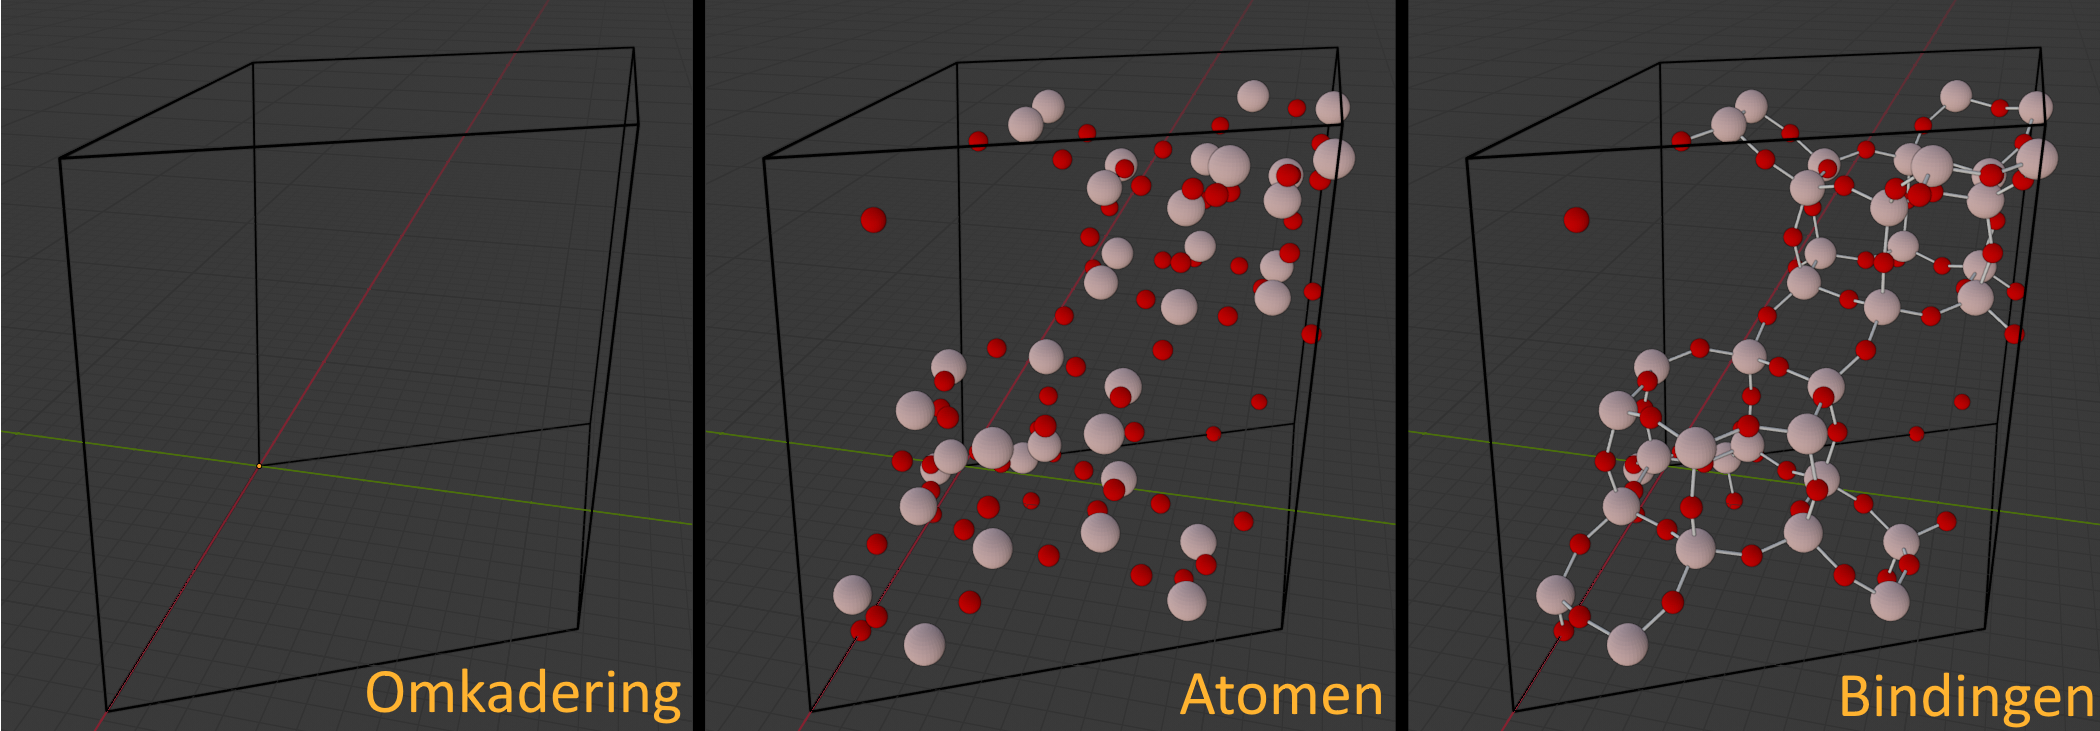
\includegraphics[width=\textwidth,keepaspectratio]{getekend.png}
\caption{De drie stappen in het tekenen van een kristal}
\end{figure}

\section{Creëren van een Blender add-on}

\subsection{Blender add-ons}
De laatste stap in het ontwerpproces is het aanmaken van een interface tussen de gebruker en het programma zodat de gebruiker op een eenvoudige manier zijn CIF-bestanden kan visualiseren. Blender laat toe zelf add-ons te creëren. Zo een add-on is een programma dat in de Blender interface kan worden opgeroepen door op de F3 toets de drukken, het is zelfs mogelijk een add-on een eigen venster te geven of in een reeds bestaand venster in te voegen.
\par
Het schrijven van een add-on kan worden gedaan in de Scripting omgeving van Blender, waar het meteen kan uitgevoerd worden of in een externe IDE zodat deze later kan worden geïnstalleerd. Een add-on hoeft slechts een keer geïnstalleerd worden en kan vanaf dan worden herladen door de \textit{Reload Scripts} functionaliteit uit te voeren in Blender. Op deze wijze kan een externe IDE gebruikt worden, welke veel handiger in omgang is dan de text editor van Blender zelf, terwijl de add-on constant kan getest worden na elke aanpassing van het script.

\subsection{Opbouw van een add-on script}
Een Blender add-on moet steeds een bestand bevatten met de naam \textit{\_\_init\_\_.py}, dit is het bestand dat Blender eerst zal uitvoeren wanneer de add-on wordt aangemaakt. In dit bestand staat steeds een header gedeelte dat \textit{bl\_info} heet. Deze variabele is een dictionary waarin de details van de add-on worden vermeld, waaronder de naam van de add-on, de versie van Blender waarvoor deze is gemaakt, de naam van de auteur en in welke editor omgeving deze add-on kan worden gebruikt. Een header is nog niet genoeg om een werkende aad-on te hebben, bij het uitvoeren van een add-on gaat Blender zoeken naar een \textit{register} methode. Deze functie zal telkens worden opgeroepen wanneer Blender de add-on zal inladen, in deze functie worden alle onderdelen van de add-on ingeladen. Deze onderdelen worden in de volgende secties verder beschreven. Wanneer de add-on wordt uitgeschakeld zal de \textit{unregister} methode worden opgeroepen welke het tegenovergestelde doet van de eerder beschreven \textit{register} methode.
\par
\subsection{Operatoren}
Operatoren, of \textit{operators}, zijn klassen in een add-on waarin de uitvoerbare elementen worden beschreven. Deze bevatten telkens hun eigen \textit{register} en \textit{unregister} methodes. In de \textit{register} methode worden de attributen van de operator beschreven, welke Blender zal aanmaken bij het inladen van de add-on. Deze attributen kunnen dan eventueel uit het geheugen worden verwijderd bij het uitvoeren van de \textit{unregister} methode wanneer de add-on wordt uitgeschakeld. 
\par
Een operator kan ook een \textit{execute} methode bevatten, deze methode zal worden opgeroepen wanneer deze operator in de add-on wordt uitgevoerd. In deze methode kunnen de attributen worden aangepast of ingelezen, kunnen andere functies worden opgeroepen of kan code staan die moet worden uitgevoerd zodra de operator wordt opgeroepen.
\par
In het programma worden twee operators aangemaakt. Eén operator heeft als functie een bestandsbrowser te openen waarmee de gebruiker het CIF-bestand kan selecteren dat moet worden gevisualiseerd. De tweede operator voert het hele script uit dat in dit hoofdstuk beschreven wordt, vanaf het converteren van het bestand met OpenBabel tot het tekenen van het kristal in Blender. Deze operatorklasse heeft een groot aantal attributen die de gebruiker kan aanpassen, waaronder enkele \textit{booleans} die kunnen aan of uitgezet worden, een \textit{float} die de maximal bindingdsafstand van de atomen bepaalt en twee \textit{enumarations} die de tekenwijze en de kwaliteit van het tekenen bepalen. Een enumeratie is een datastructuur die een verzameling is van symbolische namen, of leden, die gebonden zijn aan unieke, constante waarden. Binnen een enumeration kunnen de leden met elkaar worden vergeleken en kan er over de leden worden geïtereerd.\citep*{ENUM} Het nut van deze enumerations komt in de volgende sectie aan bod.

\subsection{Panelen}
Panelen, of \textit{panels} zijn klassen die als voornaamste functie het visualiseren van de add-on op het Blender scherm hebben. Een paneelklasse heeft enkele attributen die onder andere de naam van het paneel, in welke omgeving en in welk venster de add-on wordt weergegeven. Ook deze klasse bevat een \textit{register} en \textit{unregister} methode, om het paneel te initialiseren. Hiernaast is er nog de \textit{draw} methode, waarin de lay-out van het paneel kan worden aangepast. Hiermee kunnen de attributen van de operatoren worden weergegeven zodat ze door de gebruiker kunnen worden aangepast. Booleans worden weergegeven als selectievakjes, getallen als schuifbalken en tekstvakjes en de eerder vernoemde enumeraties als een keuzelijst van de elementen die het bevat. Hiernaast kunnen er labels gemaakt worden waarin tekst kan worden afgebeeld en worden de operators als een drukknop weergegeven die hun \textit{execute} methode uitvoert wanneer de gebruiker op deze knop klikt.
\par
De opmaak van het paneel kan worden aangepast door middel van kleuren, pictogrammen, het invoegen van scheidingen, het gebruik van rijen en kolommen en door onderdelen van het paneel in aparte kaders onder te brengen.
\par
\begin{figure}[H]
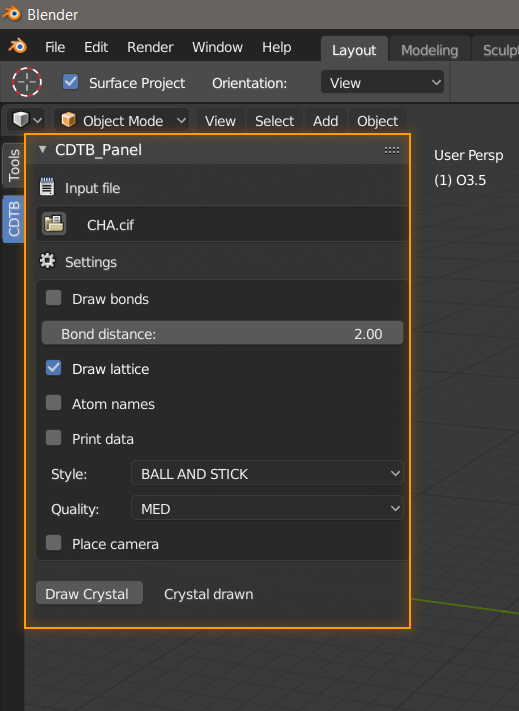
\includegraphics[scale=0.9]{paneel.png}
\caption{Het paneel van de add-on in de Blender GUI}
\end{figure}

\newpage
Het paneel van de add-on van het programma, Figuur[3.4], is terug te vinden in de \textit{3D view} omgeving van Blender onder het \textit{Tools} venster. Hiernaast is de add-on enkel zichtbaar wanneer de gebruiker zich in \textit{Object mode} bevindt. Het paneel zelf wordt opgedeeld in twee kaders. In de eerste kader staat een drukknop, die de bestandsbrowseroperator uitvoert, met een mapje als pictogram. Naast deze knop staat een label die het pad naar het geselecteerde bestand laat zien. In de tweede kader zijn alle instellingen zichtbaar die invloed hebben op het tekenen van het kristal. Hier zijn onder andere de twee keuzelijsten weergegeven.  Het veld onder de kaders is opgedeeld in twee kolommen, in de eerste kolom staat de drukknop \textit{Draw Crystal}, die de tweede operator zal uitvoeren waarmee het kristal zal getekend worden. Rechts van deze knop staat nog een label die eventuele opmerkingen aan de gebruiker zal geven, bijvoorbeeld wanneer het kristal is getekend of wanneer de er op de knop wordt geklikt zonder dat er een bestand is geselecteerd.




\section{Conclusie}
In dit hoofdstuk werden het ontwerpproces en de werking van het programma op een beknopte manier beschreven. Er werd kennisgemaakt met OpenBabel en hoe deze in het programma wordt gebruikt om de symmetrie binnen een kristal om te zetten naar een beter leesbaar formaat. Er is dieper ingegaan over hoe PyCIFRW de kristaldata uit CIF-files beschikbaar stelt in de vorm van een dictionary en hoe deze verder in worden gevuld in de geschikte klasse.
\par
Om het kristal correct te visualiseren is er nood aan een conversiematrix die de fractionele coördinaten kan omzetten naar orthogonale. Met behulp van deze matrix zal eerst een omkadering van het eenheidskristal getekend worden. Dit wordt gedaan door cilinders te tekenen tussen de hoekpunten van de cel. Vervolgens worden de atomen een voor een getekend als gekleurde bollen met verschillende afmetingen op basis van het element. Ten slotte worden de afstanden tussen de atomen berekend zodat er al dan niet een binding kan worden getekend worden.
\par
Het maken van een add-on in Blender laat de gebruiker toe het script op een eenvoudige manier uit te voeren, al dan niet met behulp van een grafische tool. Een add-on bestaat uit een header met informatie over de add-on, één of meerdere operatorklassen die attributen kunnen bezitten en een bepaalde functie uitvoeren wanneer ze worden opgeroepen en een paneelklasse waarmee het visuele aspect van de add-on kan worden gepersonaliseerd. Op zo een paneel kunnen de attributen door de gebruiker worden aangepast en kunnen de operatoren worden uitgevoerd via drukknoppen.  



 



  







%%%%%%%%%%%%%%%%%%%%%%%%%%%%%%%%%%%%%%%%%%%%%%%%%%%%%%%%%%%%%%%%%%% 
%                                                                 %
%                           INLEIDING                             %
%                                                                 %
%%%%%%%%%%%%%%%%%%%%%%%%%%%%%%%%%%%%%%%%%%%%%%%%%%%%%%%%%%%%%%%%%%% 


\chapter{Werking van het programma}

In hoofdstuk drie wordt een algemeen overzicht gegeven van de opbouw en werking van het programma. Er wordt echter niet dieper ingegaan op de onderliggende code van het programma. Dit hoofdstuk zal zich voornamelijk verdiepen in deze code, de structuur ervan en zullen de belangrijkste onderdelen ervan worden uitgelegd. Hiernaast zal er ook worden beschreven hoe de externe programma's moeten worden geïnstalleerd en hoe deze in het programma worden geïmplementeerd. 
\par
Om de gedachtegang achter het ontwerpproces makkelijker volgbaar te maken zal er in dit hoofdstuk vooral gebruikt gemaakt worden van een actieve schrijfwijze en de wetenschappelijke 'we'-vorm. De code zal worden uitgelegd aan de hand van listings die rechtstreeks uit de code van het programma komen. De volledige code kan worden teruggevonden in de bijlages van deze tekst.[Bijlage D]
\par


\section{Installatie van externe programma's}
Zoals in hoodstuk drie wordt beschreven gaan we gebruik maken van twee externe programma's die we zullen nodig zullen hebben om het programma uit te kunnen voeren, OpenBabel en PyCIFRW. Deze sectie legt uit hoe we deze kunnen installeren op een systeem. Hoewel deze in het geval van dit onderzoek met Windows 10 wordt gewerkt, werken deze software ook op oudere versies van Windows. Ons programma is gericht op besturingssysteemonafhankelijkheid, dit wil zeggen dat het ook op Linux en Apple moet werken. Het is echter mogelijk dat het installeren van deze externe programma's anders verloopt dan op Windows. De installatie van deze programma's zal in deze tekst echter enkel voor Windowssytemen worden uitgelegd.

\subsection{OpenBabel}  
De installatie van OpenBabel kan gevonden worden op hun webpagina: \url{http://openbabel.org/wiki/Category:Installation} en is gratis voor iedereen. Op deze pagina gaan we de OpenBabelGUI \textit{installer} downloaden, zie Figuur[4.1], let op dat de bit-versie met die van ons systeem overeenkomt. De download zou automatisch moeten starten. Ten slotte kunnen we de installatiewizard starten door het gedownloade bestand uit te voeren.
\par
Na het volgen van de installatiewizard zou de OpenBabel GUI moeten geïnstalleerd zijn op ons systeem, en kan het gebruikt worden in ons programma. Dit zal in het verdere verloop van dit hoofdstuk worden uitgelegd.

\subsection{PyCIFRW}
Voor de PyCIFRW module op ons systeem te installeren hebben we nood aan een prompt waarop Pyhton3.7 kan worden uitgevoerd. Zo'n prompt kan verkregen worden door anaconda te installeren en gebruik te maken van \textit{Anaconda prompt}. Vervolgens hebben we de pip installer nodig voor Python en is automatisch aanwezig op Python3.7
\par 
Pip laat ons toe allerlei Python modules te installeren, waaronder de PyCIFRW module. Dit doen we met door volgend commando in te geven in het prompt:
\begin{lstlisting}[caption=,numbers=none,language= bash]
  pip install PyCifRW
\end{lstlisting}
Dit zorgt ervoor dat we nu toegang hebben tot de PyCIFRW module wanneer we Python uitvoeren en kan eenvoudig getest worden door Python op te starten en het volgende lijn code uit te voeren:
\begin{lstlisting}[caption=,numbers=none]
  import CifFile
\end{lstlisting}

Als er geen foutmelding wordt gegeven wilt het zeggen dat de module correct is geïnstalleerd op voor onze Python installatie. 
\par
Doordat Blender een eigen Python installatie heeft zal deze nog geen toegang hebben tot onze geïnstalleerde modules. Dit kunnen we oplossen door de map die de PyCIFRW module bevat te kopiëren naar de Python installatie van Blender. Deze map kunnen we vinden op plaats waar we Python hebben geïnstalleerd op ons systeem, in het geval dat Anaconda wordt gebruikt vinden we deze in de installatiemap van Anaconda in de submap \textit{site-packages} (Anaconda3 \textgreater \textgreater{} Lib \textgreater \textgreater{} site-packages).
Vervolgens moeten we de map \textit{CifFile} kopiëren naar de Python installatie van Blender (blender-2.80.0-git.3c8c1841d72-windows64 \textgreater \textgreater{} 2.80 \textgreater \textgreater{} python \textgreater \textgreater{} lib \textgreater \textgreater{} site-packages). 
\par
Een alternatieve methode om de PyCIFRW module werkende te krijgen op Blender, zonder nood te hebben aan een Python3.7 installatie, is door de \textit{CifFile} map rechtstreeks in de Pythoninstallatiemap van Blender te plaatsen. De \textit{CifFile} kan gedownload worden vanaf de GitHub pagina van deze thesis: \url{https://github.com/JarritB/Thesis}
\par
  

% Bibliografie: referenties. De items zitten in bibliografie.bib
%%%%%%%%%%%%%%%%%%%%%%%%%%%%%%%%%%%%%%%%%%%%%%%%%%%%%%%%%%%%%%%%%
% Indien je ook de niet geciteerde werken in je bibliografie wil opnemen, commentarieer dan onderstaande regel uit!
\nocite{*}
\bibliographystyle{apalike}
\bibliography{bibliografie}

% Eventueel enkele appendices
%%%%%%%%%%%%%%%%%%%%%%%%%%%%%%
\appendix
\chapter{Uitleg over de appendices}
Bijlagen worden bij voorkeur enkel elektronisch ter beschikking gesteld. Indien essentieel kunnen in overleg met de promotor bijlagen in de scriptie opgenomen worden of als apart boekdeel voorzien worden.

Er wordt wel steeds een lijst met vermelding van alle bijlagen opgenomen in de scriptie. Bijlagen worden genummerd het een drukletter A, B, C,...

Voorbeelden van bijlagen:\\
Bijlage A: \qquad	Detailtekeningen van de proefopstelling \\
Bijlage B: \qquad	Meetgegevens (op USB)
\\





% Back cover: change according to the correct campus

\includepdf{private/back_fiiw_denayer.pdf}
\chapter*{Grantt Map: Actuele Planning}
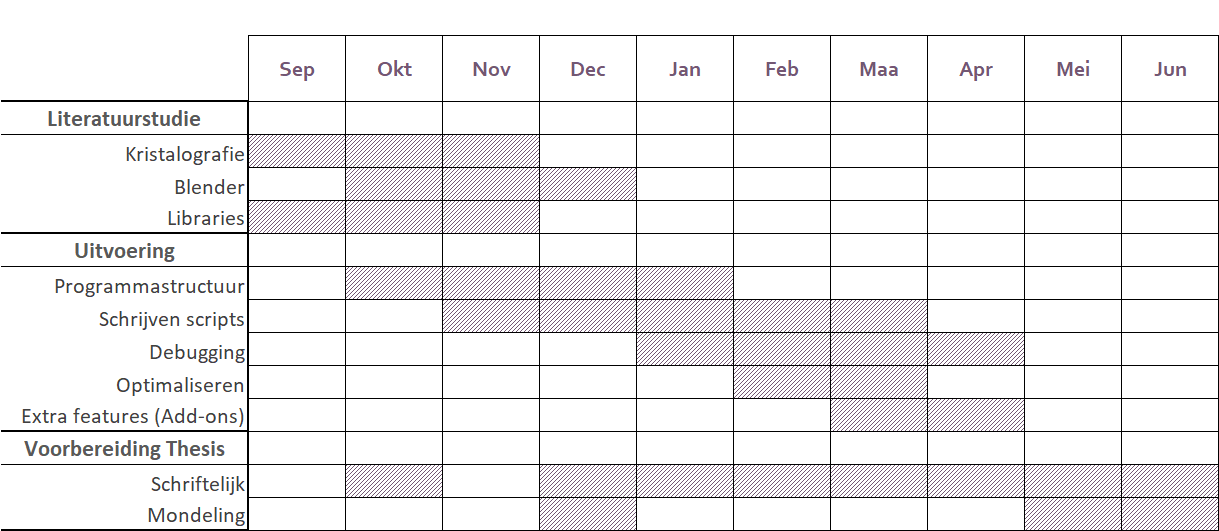
\includegraphics[width=\textwidth,height=\textheight,keepaspectratio]{Grantt.png}
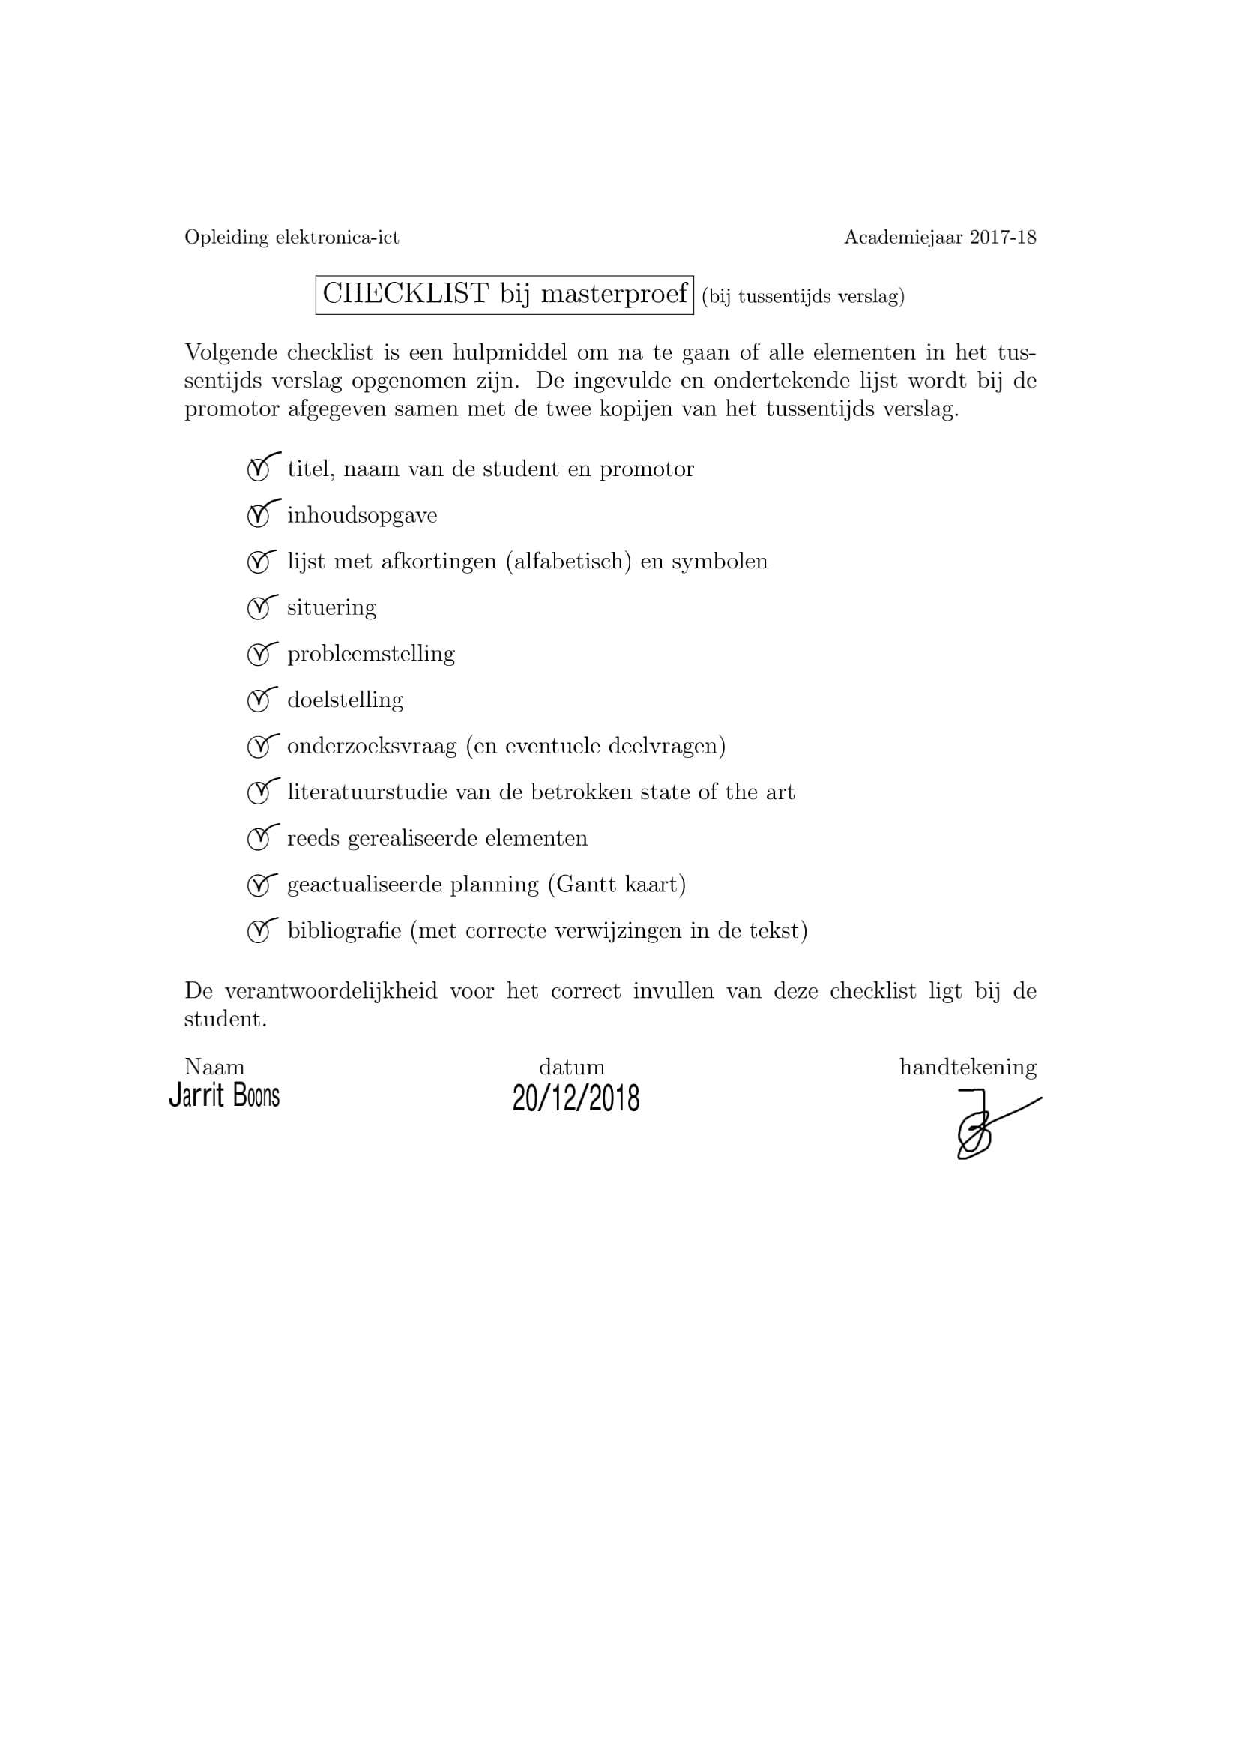
\includepdf{checklist.pdf}



\end{document}
